\documentclass[hyperref={bookmarks=false},aspectratio=169]{beamer}
\usepackage{hyperref,ragged2e,amsmath,amssymb,url,bm}
\usepackage{graphicx,booktabs,array}
\usepackage{tikz}
\usetikzlibrary{shadows}
\usetikzlibrary{arrows.meta,positioning,calc,shapes.geometric,decorations.pathreplacing,matrix}
\graphicspath{{crops/}}
\usetheme{Goettingen}
% --- Paleta "Israel": celeste y azul del tejelet (Nm 15:38), oro del santuario, fondo crema ---
% (los nombres de color se conservan por compatibilidad con los cuerpos de las láminas: «ladrillo» = azul tejelet,
%  «cafe» = azul real, «cafeosc» = azul noche, «piedra» = celeste claro, «sepia» = azul pizarra)
\definecolor{cafe}{RGB}{26,82,150}
\definecolor{cafeosc}{RGB}{11,33,74}
\definecolor{tinta}{RGB}{20,32,56}
\definecolor{oro}{RGB}{206,162,52}
\definecolor{ladrillo}{RGB}{20,68,140}
\definecolor{piedra}{RGB}{234,243,251}
\definecolor{sepia}{RGB}{72,102,140}
\definecolor{celeste}{RGB}{96,166,222}
\setbeamercolor{structure}{fg=ladrillo}
\setbeamertemplate{sidebar canvas right}[vertical shading][top=celeste!75!ladrillo,middle=ladrillo,bottom=cafeosc]
\setbeamercolor{title in sidebar}{fg=oro!80!white}
\setbeamercolor{author in sidebar}{fg=piedra}
\setbeamercolor{section in sidebar}{fg=white}
\setbeamercolor{section in sidebar shaded}{fg=celeste!45!white}
\setbeamercolor{subsection in sidebar}{fg=white}
\setbeamercolor{subsection in sidebar shaded}{fg=celeste!45!white}
\let\raggedright\justifying
\definecolor{crema}{RGB}{250,245,230}
\setbeamertemplate{background canvas}[default]
\setbeamercolor{background canvas}{bg=crema}
\setbeamercolor{normal text}{fg=tinta}
\setbeamercolor{frametitle}{fg=ladrillo}
\setbeamerfont{frametitle}{series=\bfseries}
\setbeamertemplate{section in toc shaded}{\leavevmode{\color{sepia!85!black}\inserttocsection}\par}
\setbeamercolor{title}{fg=ladrillo}
\setbeamercolor{subtitle}{fg=cafe}
\setbeamercolor{item projected}{bg=cafe,fg=piedra}
\setbeamertemplate{itemize item}{\small\textcolor{oro!85!ladrillo}{$\blacktriangleright$}}
\setbeamertemplate{navigation symbols}{}
% --- Español + hebreo + griego (XeLaTeX) con fuentes empaquetadas en fonts/ ---
\usepackage[bidi=default]{babel}
\babelprovide[import,main]{spanish}
\babelprovide[import]{hebrew}
\babelprovide[import]{ancientgreek}
\babelfont[hebrew]{sf}[Path=fonts/, BoldFont=NotoHebrewSans-700.ttf]{NotoHebrewSans-400.ttf}
\babelfont[hebrew]{rm}[Path=fonts/, BoldFont=NotoHebrewSans-700.ttf]{NotoHebrewSans-400.ttf}
\babelfont[ancientgreek]{sf}[Path=fonts/]{GFSPorson.otf}
\babelfont[ancientgreek]{rm}[Path=fonts/]{GFSPorson.otf}
\newcommand{\heb}[1]{\mbox{\foreignlanguage{hebrew}{#1}}}
\newcommand{\grc}[1]{\foreignlanguage{ancientgreek}{#1}}
% --- Citas, imágenes, referencias ---
\usepackage[most]{tcolorbox}
\newtcolorbox{cita}[1][]{enhanced, colback=piedra!92!white, colframe=oro!90!ladrillo,
  boxrule=0pt, leftrule=2.5pt, arc=0pt, left=6pt, right=6pt, top=4pt, bottom=4pt,
  before skip=4pt, after skip=6pt, fontupper=\small\itshape, #1}
\newcommand{\fuente}[1]{\par\hfill{\upshape\bfseries\footnotesize\textcolor{ladrillo}{#1}}}
\newcommand{\imagen}[3][0.80]{%
  \centering\includegraphics[height=#1\textheight,width=\linewidth,keepaspectratio]{#2}\par\vspace{2pt}
  {\fontsize{5}{6}\selectfont\color{sepia}{\raggedleft\textit{Nota.} #3\par}}}
\makeatletter
\newcommand{\fotolado}[2]{%
  % Panel a la derecha, separado de la columna de texto (0.57): marco dorado, sombra y nota al pie.
  \begin{tikzpicture}[remember picture,overlay]
    \coordinate (fl) at ([xshift=\beamer@leftmargin+0.615\textwidth]current page.west);
    \coordinate (fr) at ([xshift=-\beamer@sidebarwidth-6pt]current page.east);
    \node[inner sep=0pt,anchor=center,draw=oro,line width=0.9pt,
      drop shadow={shadow xshift=1.2pt,shadow yshift=-1.2pt,opacity=0.30,fill=cafeosc}] (foto)
      at ([yshift=6pt]$(fl)!0.5!(fr)$)
      {\includegraphics[width=\dimexpr\paperwidth-\beamer@sidebarwidth-\beamer@leftmargin-0.615\textwidth-6pt\relax]{#1}};
    \node[anchor=north east,inner sep=0pt,text=sepia,font=\fontsize{4.6}{5.6}\selectfont,align=right,
      text width=\dimexpr\paperwidth-\beamer@sidebarwidth-\beamer@leftmargin-0.615\textwidth-6pt\relax]
      at ([yshift=-3pt]foto.south east) {\textit{Nota.} #2};
  \end{tikzpicture}}
\makeatother
\newcommand{\refapa}[1]{\par\hangindent=1.2em\hangafter=1\noindent #1\par\vspace{3pt}}
\usepackage{xurl}\urlstyle{same}
\newcommand{\destacar}[1]{\textbf{\textcolor{ladrillo}{#1}}}
% --- Piezas visuales de la serie: regla dorada bajo el título, notas y pies de figura ---
\addtobeamertemplate{frametitle}{}{\vspace{-3pt}{\color{oro}\rule{2.2cm}{1.1pt}}\vspace{1pt}}
\newtcolorbox{notalam}[1][Nota]{enhanced,colback=oro!10!white,colframe=oro!85!ladrillo,boxrule=0.5pt,arc=2pt,
  left=5pt,right=5pt,top=3pt,bottom=3pt,fonttitle=\bfseries\scriptsize,coltitle=cafeosc,colbacktitle=oro!30!white,
  fontupper=\scriptsize,title={#1},before skip=4pt,after skip=4pt}
\newtcolorbox{clave}[1][]{enhanced,colback=piedra,colframe=ladrillo,boxrule=0pt,leftrule=2.5pt,arc=0pt,
  left=5pt,right=5pt,top=3pt,bottom=3pt,fontupper=\scriptsize,before skip=4pt,after skip=4pt,#1}
\newcommand{\notafig}[1]{\par\vspace{2pt}{\fontsize{5}{6}\selectfont\color{sepia}\hfill\textit{Nota.} #1\par}}
\newcommand{\elabpropia}{\notafig{Elaboración propia.}}
\tikzset{hito/.style={circle,fill=oro,draw=white,line width=0.6pt,inner sep=1.6pt},
  etiq/.style={font=\tiny,text=tinta,align=center},
  flecha/.style={->,draw=oro!90!ladrillo,line width=1pt},
  bloque/.style={draw=ladrillo,line width=0.6pt,fill=piedra,rounded corners=3pt,font=\scriptsize,align=center,inner sep=4pt},
  bloqueoro/.style={draw=oro!90!ladrillo,line width=0.6pt,fill=oro!14!white,rounded corners=3pt,font=\scriptsize,align=center,inner sep=4pt},
  bloqueazul/.style={draw=cafeosc,fill=ladrillo,text=white,rounded corners=3pt,font=\scriptsize\bfseries,align=center,inner sep=4pt}}

\tikzset{caja/.style={draw=cafe!80!black,line width=0.7pt,top color=piedra!55!white,bottom color=piedra!92!oro,
  rounded corners=4pt,inner sep=5pt,font=\scriptsize,
  drop shadow={shadow xshift=0.7pt,shadow yshift=-0.8pt,opacity=0.25,fill=cafeosc}},
  >={Stealth[length=2.4mm,width=1.8mm]}, every picture/.style={line cap=round,line join=round}}
\newcommand{\precision}[1]{{\footnotesize\color{sepia}\textbf{Precisión:} #1}}
\newcommand{\pt}[2]{({#1-30},{#2-29})}
% AVISO: este archivo incluye la sección «Análisis exegético pasaje por pasaje» (11:1-36, «ahora» de 11:30-31, «y así», «de Sion») y la predicación «El misterio revelado». Editar siempre sobre main actualizado (git pull); no regenerar desde copias antiguas.
\title[Israel 8: Romanos 11]{\bfseries{Israel, el pueblo de Dios}}
\subtitle{Estudio 8. Romanos 11: la restauración de Israel}
\author{}\institute{}\date{}
\titlegraphic{
\includegraphics[width=0.85\linewidth,height=0.38\textheight,keepaspectratio]{portada.jpg}\\[-1pt]
  {\fontsize{5}{6}\selectfont\color{sepia}\textit{Nota.} Elaboración propia: Ro 11:26a en escritura uncial (texto NA28).}}
\newcommand{\mpt}[2]{({(#1-12)*0.26},{(#2-30)*0.33})}
\begin{document}
\frame{\titlepage}

% ===================================================
\section{Introducción}
\begin{frame}{¿Ha desechado Dios a su pueblo?}
\begin{columns}[T,onlytextwidth]
\begin{column}{0.52\textwidth}
\begin{cita}Digo, pues: ¿Ha desechado Dios a su pueblo? ¡De ningún modo! Porque también yo soy israelita, de la descendencia de Abraham, de la tribu de Benjamín. No ha desechado Dios a su pueblo, al cual conoció de antemano.\fuente{(Ro 11:1--2)}\end{cita}
\begin{cita}Porque irrevocables son los dones y el llamamiento de Dios.\fuente{(Ro 11:29)}\end{cita}
\end{column}
\begin{column}{0.45\textwidth}
\centering
\begin{tikzpicture}[node distance=0.32cm]
\node[bloque,text width=5.2cm] (a) {Roma, c. 57 e.\,c.: la mayoría de Israel no cree en Jesús; crecen las iglesias de gentiles};
\node[bloqueoro,text width=5.2cm,below=of a] (b) {Tentación: concluir que \textbf{Dios cambió de pueblo}};
\node[bloqueazul,text width=5.2cm,below=of b] (c) {\grc{μὴ γένοιτο}: «¡de ningún modo!» (11:1)};
\node[bloque,text width=2.35cm,below=0.45cm of c.south west,anchor=north west] (d) {\textbf{Identidad}\\{\tiny un remanente preserva la vocación (11:5, 29)}};
\node[bloque,text width=2.35cm,below=0.45cm of c.south east,anchor=north east] (e) {\textbf{Restauración}\\{\tiny «y así todo Israel será salvo» (11:26)}};
\draw[flecha] (a) -- (b); \draw[flecha] (b) -- (c);
\draw[flecha] (c.south) -- ++(0,-0.2) -| (d.north);
\draw[flecha] (c.south) -- ++(0,-0.2) -| (e.north);
\end{tikzpicture}\elabpropia
\end{column}
\end{columns}
\end{frame}

\begin{frame}{La culminación de la serie}
\centering
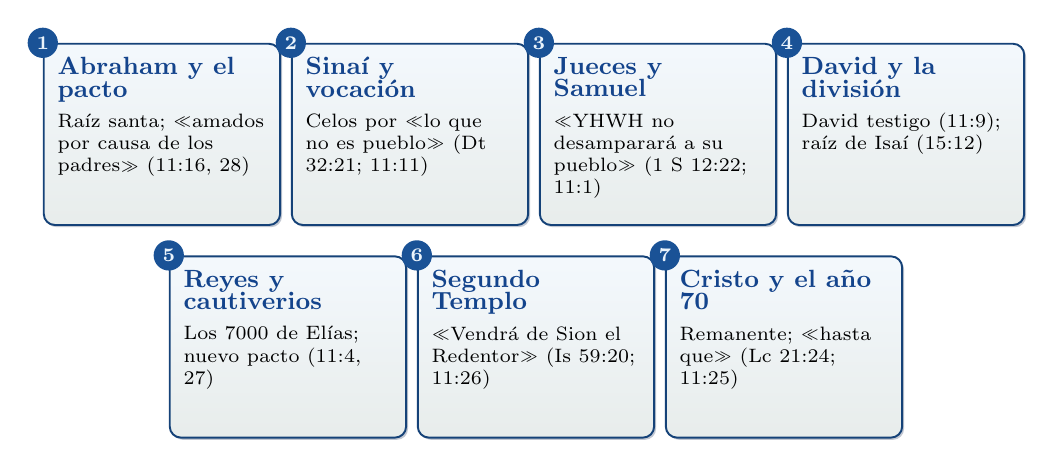
\begin{tikzpicture}
 \foreach \x/\y/\n/\t/\r in {0/0/1/{Abraham y el pacto}/{Raíz santa; «amados por causa de los padres» (11:16, 28)},
   3.15/0/2/{Sinaí y vocación}/{Celos por «lo que no es pueblo» (Dt 32:21; 11:11)},
   6.3/0/3/{Jueces y Samuel}/{«YHWH no desamparará a su pueblo» (1~S 12:22; 11:1)},
   9.45/0/4/{David y la división}/{David testigo (11:9); raíz de Isaí (15:12)},
   1.6/-2.7/5/{Reyes y cautiverios}/{Los 7000 de Elías; nuevo pacto (11:4, 27)},
   4.75/-2.7/6/{Segundo Templo}/{«Vendrá de Sion el Redentor» (Is 59:20; 11:26)},
   7.9/-2.7/7/{Cristo y el año 70}/{Remanente; «hasta que» (Lc 21:24; 11:25)}}{
  \node[caja,anchor=north] (b\n) at (\x,\y) {\parbox[t][1.95cm][t]{2.65cm}{\RaggedRight
    {\small\textbf{\textcolor{ladrillo}{\t}}}\\[3pt]\scriptsize \r}};
  \node[circle,fill=cafe,text=piedra,font=\scriptsize\bfseries,inner sep=1.6pt] at (b\n.north west) {\n};}
\end{tikzpicture}\par\vspace{4pt}
{\small\itshape\color{sepia}En Romanos 11 desembocan los siete estudios anteriores: el capítulo recoge una historia ya escrita.}
\elabpropia
\end{frame}

\begin{frame}{Cuatro dimensiones}
\centering
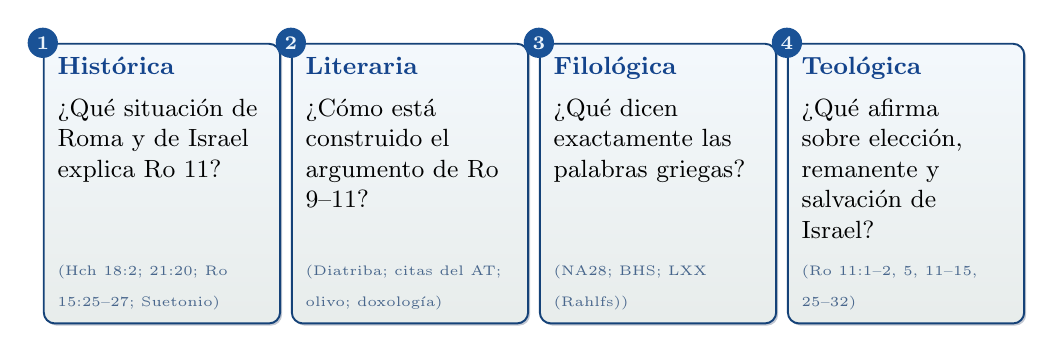
\begin{tikzpicture}
 \foreach \x/\n/\t/\d/\r in {0/1/{Histórica}/{¿Qué situación de Roma y de Israel explica Ro 11?}/{Hch 18:2; 21:20; Ro 15:25--27; Suetonio},
   3.15/2/{Literaria}/{¿Cómo está construido el argumento de Ro 9--11?}/{Diatriba; citas del AT; olivo; doxología},
   6.3/3/{Filológica}/{¿Qué dicen exactamente las palabras griegas?}/{NA28; BHS; LXX (Rahlfs)},
   9.45/4/{Teológica}/{¿Qué afirma sobre elección, remanente y salvación de Israel?}/{Ro 11:1--2, 5, 11--15, 25--32}}{
  \node[caja,anchor=north] (b\n) at (\x,0) {\parbox[t][3.2cm][t]{2.65cm}{\RaggedRight
    {\small\textbf{\textcolor{ladrillo}{\t}}}\\[4pt]\small \d\par\vfill{\tiny\color{sepia}(\r)}}};
  \node[circle,fill=cafe,text=piedra,font=\scriptsize\bfseries,inner sep=1.6pt] at (b\n.north west) {\n};}
\end{tikzpicture}\elabpropia
\begin{notalam}[Traducción, numeración y el nombre «Israel»]
Citas bíblicas: traducción propia desde el hebreo (BHS) y el griego (NA28); LXX según Rahlfs-Hanhart. Numeración española [hebrea o griega] cuando difiere. En Ro 9--11, «Israel» es siempre el \textbf{pueblo completo}, nunca el antiguo reino del norte; cuando se hable del reino del norte (Efraín, Samaria) o de Judá (Jerusalén) se dirá expresamente.
\end{notalam}
\end{frame}

% ===================================================
\section{Historia}
\begin{frame}{Roma y la carta: cronología}
\centering\vspace*{-4pt}
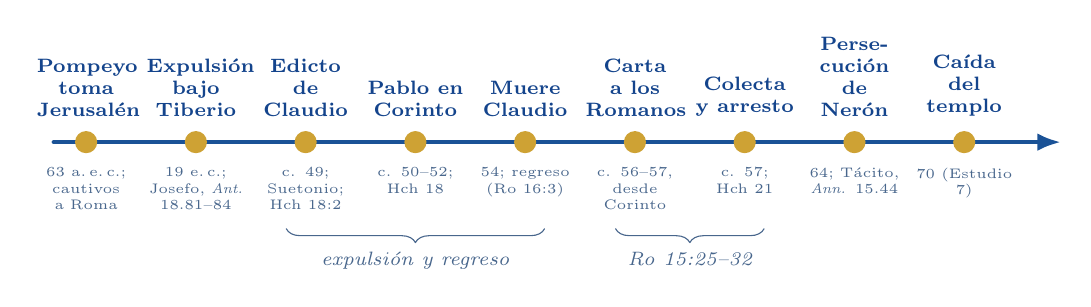
\begin{tikzpicture}[x=0.82cm]
\draw[line width=1.6pt,cafe,-{Latex[length=3mm]}] (0,0) -- (15.6,0);
\foreach \x/\t/\b in {0.5/{Pompeyo toma Jerusalén}/{63 a.\,e.\,c.; cautivos a Roma},
                      2.2/{Expulsión bajo Tiberio}/{19 e.\,c.; Josefo, \emph{Ant.} 18.81--84},
                      3.9/{Edicto de Claudio}/{c. 49; Suetonio; Hch 18:2},
                      5.6/{Pablo en Corinto}/{c. 50--52; Hch 18},
                      7.3/{Muere Claudio}/{54; regreso (Ro 16:3)},
                      9.0/{Carta a los Romanos}/{c. 56--57, desde Corinto},
                      10.7/{Colecta y arresto}/{c. 57; Hch 21},
                      12.4/{Perse\-cución de Nerón}/{64; Tácito, \emph{Ann.} 15.44},
                      14.1/{Caída del templo}/{70 (Estudio 7)}}{
  \fill[oro] (\x,0) circle (4pt);
  \node[above,font=\scriptsize\bfseries,text=ladrillo,text width=1.25cm,align=center] at (\x,0.2) {\t};
  \node[below,font=\tiny,text=sepia,text width=1.25cm,align=center] at (\x,-0.2) {\b};}
\draw[decorate,decoration={brace,amplitude=5pt,mirror},sepia] (3.6,-1.1) -- (7.6,-1.1) node[midway,below=5pt,font=\scriptsize\itshape]{expulsión y regreso};
\draw[decorate,decoration={brace,amplitude=5pt,mirror},sepia] (8.7,-1.1) -- (11.0,-1.1) node[midway,below=5pt,font=\scriptsize\itshape]{Ro 15:25--32};
\end{tikzpicture}\par
{\fontsize{5}{6}\selectfont\color{sepia}\raggedleft\textit{Nota.} Elaboración propia. Fechas aproximadas.\par}
\begin{notalam}[Precisión arqueológica: Galión y Erasto]
\textbf{Galión} (inscripción de Delfos): procónsul de Acaya c. 51--52; fecha la estancia de Pablo en Corinto (Hch 18:12). \textbf{Erasto} (pavimento de Corinto): edil; su identificación con el de Ro 16:23 \textbf{está en debate} (\grc{οἰκονόμος} no equivale a \emph{aedilis}).
\end{notalam}
\end{frame}

\begin{frame}{Corinto, Roma y Jerusalén}
\begin{columns}[c,onlytextwidth]
\begin{column}{0.66\textwidth}\centering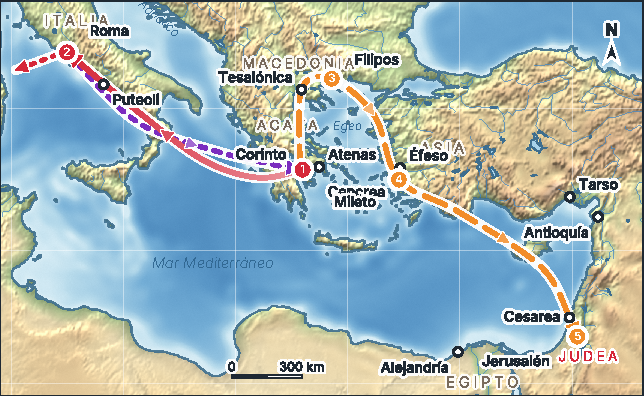
\includegraphics[width=\linewidth,height=0.86\textheight,keepaspectratio]{mapa_romanos.pdf}\par\vspace{1pt}{\fontsize{4.5}{5.5}\selectfont\color{sepia}\textit{Nota.} Elaboración propia (GSHHS/WDB, Basemap); ubicaciones aproximadas.\par}\end{column}
\begin{column}{0.32\textwidth}\scriptsize\RaggedRight
{\scriptsize\RaggedRight
\definecolor{mapacarmesi}{HTML}{D62839}
\definecolor{mapanaranja}{HTML}{F28C28}
\definecolor{mapavioleta}{HTML}{7B2CBF}
\definecolor{mapaturquesa}{HTML}{0F8B8D}
\definecolor{mapaazul}{HTML}{1D4E89}
\definecolor{mapaocre}{HTML}{B5651D}
\tikz[baseline=-0.6ex]{\draw[white,line width=3.2pt,line cap=round](0,0)--(0.62,0);\draw[mapavioleta,line width=1.8pt,line cap=round,dash pattern=on 1.4pt off 1.6pt,-{Latex[length=1.6mm]}](0,0)--(0.62,0);}~Edicto de Claudio: Aquila y Priscila (Hch 18:2)\par
\tikz[baseline=-0.6ex]{\draw[white,line width=3.2pt,line cap=round](0,0)--(0.62,0);\draw[mapacarmesi,line width=1.8pt,line cap=round,-{Latex[length=1.6mm]}](0,0)--(0.62,0);}~La carta con Febe: Cencrea $\to$ Roma (Ro 16:1)\par
\tikz[baseline=-0.6ex]{\draw[white,line width=3.2pt,line cap=round](0,0)--(0.62,0);\draw[mapanaranja,line width=1.8pt,line cap=round,dash pattern=on 3.6pt off 2pt,-{Latex[length=1.6mm]}](0,0)--(0.62,0);}~La colecta: Corinto $\to$ Jerusalén (Ro 15:25–26; Hch 20–21)\par
\tikz[baseline=-0.6ex]{\draw[white,line width=3.2pt,line cap=round](0,0)--(0.62,0);\draw[mapacarmesi,line width=1.8pt,line cap=round,dash pattern=on 1.4pt off 1.6pt,-{Latex[length=1.6mm]}](0,0)--(0.62,0);}~Proyecto: hacia España (Ro 15:24, 28)\par
\smallskip{\color{black!70}\textbf{Itinerario}}\par
\tikz[baseline=-0.7ex]\node[circle,fill=mapacarmesi,draw=white,line width=0.5pt,text=white,font=\fontsize{5}{5}\selectfont\bfseries,inner sep=0.6pt,minimum size=2.6mm]{1};\,Cencrea\quad \tikz[baseline=-0.7ex]\node[circle,fill=mapacarmesi,draw=white,line width=0.5pt,text=white,font=\fontsize{5}{5}\selectfont\bfseries,inner sep=0.6pt,minimum size=2.6mm]{2};\,Roma\quad \tikz[baseline=-0.7ex]\node[circle,fill=mapanaranja,draw=white,line width=0.5pt,text=white,font=\fontsize{5}{5}\selectfont\bfseries,inner sep=0.6pt,minimum size=2.6mm]{3};\,Filipos\quad \tikz[baseline=-0.7ex]\node[circle,fill=mapanaranja,draw=white,line width=0.5pt,text=white,font=\fontsize{5}{5}\selectfont\bfseries,inner sep=0.6pt,minimum size=2.6mm]{4};\,Mileto\quad \tikz[baseline=-0.7ex]\node[circle,fill=mapanaranja,draw=white,line width=0.5pt,text=white,font=\fontsize{5}{5}\selectfont\bfseries,inner sep=0.6pt,minimum size=2.6mm]{5};\,Jerusalén\par}

\end{column}
\end{columns}
\end{frame}

\begin{frame}{Corinto, Roma y Jerusalén: claves}
\begin{columns}[T,onlytextwidth]
\begin{column}{0.40\textwidth}\small\RaggedRight
Desde \textbf{Corinto} (Hch 20:2--3; Ro 16:1, 23), Pablo escribe a una iglesia que \textbf{no fundó}.\par\medskip
Febe, de Cencrea, el puerto oriental de Corinto, lleva la carta (Ro 16:1); Pablo, la colecta a Jerusalén.\par\medskip
Aquila y Priscila habían llegado a Corinto expulsados por el edicto de Claudio (Hch 18:2).
\end{column}
\begin{column}{0.56\textwidth}
\centering
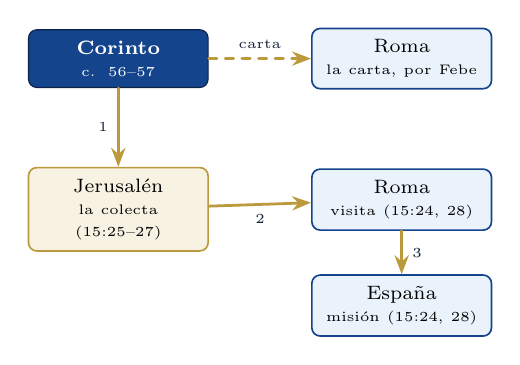
\begin{tikzpicture}[node distance=0.55cm and 0.5cm]
\node[bloqueazul,text width=2.0cm] (cor) {Corinto\\{\tiny\mdseries c. 56--57}};
\node[bloque,text width=2.0cm,right=1.3cm of cor] (rom) {Roma\\{\tiny la carta, por Febe}};
\node[bloqueoro,text width=2.0cm,below=1.0cm of cor] (jer) {Jerusalén\\{\tiny la colecta (15:25--27)}};
\node[bloque,text width=2.0cm,below=1.0cm of rom] (rom2) {Roma\\{\tiny visita (15:24, 28)}};
\node[bloque,text width=2.0cm,below=0.55cm of rom2] (esp) {España\\{\tiny misión (15:24, 28)}};
\draw[flecha,dashed] (cor) -- node[above,etiq]{carta} (rom);
\draw[flecha] (cor) -- node[left,etiq]{1} (jer);
\draw[flecha] (jer) -- node[below,etiq]{2} (rom2);
\draw[flecha] (rom2) -- node[right,etiq]{3} (esp);
\end{tikzpicture}\elabpropia
\begin{clave}La ruta explica el tono: Pablo va a Jerusalén con la ofrenda de los gentiles y escribe a Roma antes de llegar.\end{clave}
\end{column}
\end{columns}
\end{frame}

\begin{frame}{El edicto de Claudio}
\begin{columns}[T,onlytextwidth]
\begin{column}{0.50\textwidth}
\begin{cita}A los judíos, que provocaban continuos tumultos por instigación de Cresto, los expulsó de Roma.\fuente{(Suetonio, \emph{Claudio} 25.4)}\end{cita}
\begin{cita}Encontró a un judío llamado Aquila [\ldots] recién venido de Italia con Priscila su mujer, porque Claudio había mandado que todos los judíos salieran de Roma.\fuente{(Hch 18:2)}\end{cita}
\end{column}
\begin{column}{0.47\textwidth}
\centering
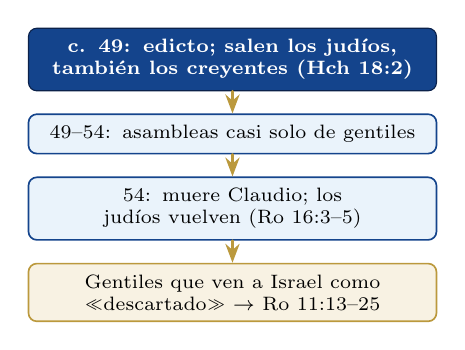
\begin{tikzpicture}[node distance=0.28cm]
\node[bloqueazul,text width=4.9cm] (a) {c. 49: edicto; salen los judíos, también los creyentes (Hch 18:2)};
\node[bloque,text width=4.9cm,below=of a] (b) {49--54: asambleas casi solo de gentiles};
\node[bloque,text width=4.9cm,below=of b] (c) {54: muere Claudio; los judíos vuelven (Ro 16:3--5)};
\node[bloqueoro,text width=4.9cm,below=of c] (d) {Gentiles que ven a Israel como «descartado» $\to$ Ro 11:13--25};
\draw[flecha] (a)--(b); \draw[flecha] (b)--(c); \draw[flecha] (c)--(d);
\end{tikzpicture}\par
{\fontsize{5}{6}\selectfont\color{sepia}\hfill\textit{Nota.} Elaboración propia a partir de Wiefel (1991).\par}
\end{column}
\end{columns}
\begin{notalam}[Cresto y la fecha]
\emph{Chrestus} y \emph{Christus} sonaban casi igual: lo probable son disputas sinagogales sobre Jesús como Mesías, aunque Cresto pudo ser un judío real. Fecha c. 49 según Orosio (7.6.15); Dión Casio (60.6.6) habla de una prohibición de reunirse en el 41. La hipótesis de Wiefel se discute en sus detalles.
\end{notalam}
\end{frame}

\begin{frame}{Remanente, colecta y arrogancia}
\begin{columns}[T,onlytextwidth]
\begin{column}{0.49\textwidth}
\begin{cita}Ya ves, hermano, cuántas \textbf{miríadas} de judíos hay que han creído, y todos son celosos de la ley.\fuente{(Hch 21:20)}\end{cita}
\begin{cita}[fontupper=\scriptsize\itshape]Si los gentiles han sido hechos \textbf{participantes} de sus bienes espirituales, deben también servirles con los materiales.\fuente{(Ro 15:27)}\end{cita}
\small \grc{ἐκοινώνησαν} (15:27) anticipa \grc{συγκοινωνός} del olivo (11:17).
\end{column}
\begin{column}{0.49\textwidth}
\centering
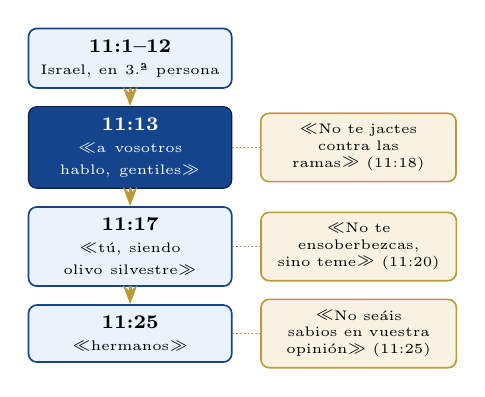
\begin{tikzpicture}[node distance=0.22cm]
\node[bloque,text width=2.3cm] (a) {\textbf{11:1--12}\\{\tiny Israel, en 3.ª persona}};
\node[bloqueazul,text width=2.3cm,below=of a] (b) {11:13\\{\tiny\mdseries «a vosotros hablo, gentiles»}};
\node[bloque,text width=2.3cm,below=of b] (c) {\textbf{11:17}\\{\tiny «tú, siendo olivo silvestre»}};
\node[bloque,text width=2.3cm,below=of c] (d) {\textbf{11:25}\\{\tiny «hermanos»}};
\foreach \u/\v in {a/b,b/c,c/d}{\draw[flecha] (\u)--(\v);}
\node[bloqueoro,text width=2.2cm,right=0.35cm of b,font=\tiny] (w1) {«No te jactes contra las ramas» (11:18)};
\node[bloqueoro,text width=2.2cm,right=0.35cm of c,font=\tiny] (w2) {«No te ensoberbezcas, sino teme» (11:20)};
\node[bloqueoro,text width=2.2cm,right=0.35cm of d,font=\tiny] (w3) {«No seáis sabios en vuestra opinión» (11:25)};
\draw[oro!80!ladrillo,densely dotted] (b)--(w1); \draw[oro!80!ladrillo,densely dotted] (c)--(w2); \draw[oro!80!ladrillo,densely dotted] (d)--(w3);
\end{tikzpicture}\elabpropia
\begin{clave}Ro 11 habla \emph{sobre} Israel, pero se dirige \emph{a} los gentiles: una corrección pastoral antes que un mapa del fin.\end{clave}
\end{column}
\end{columns}
\end{frame}

% ===================================================
\section{Literatura}
\begin{frame}{Mapa de Romanos 9--11}
\centering
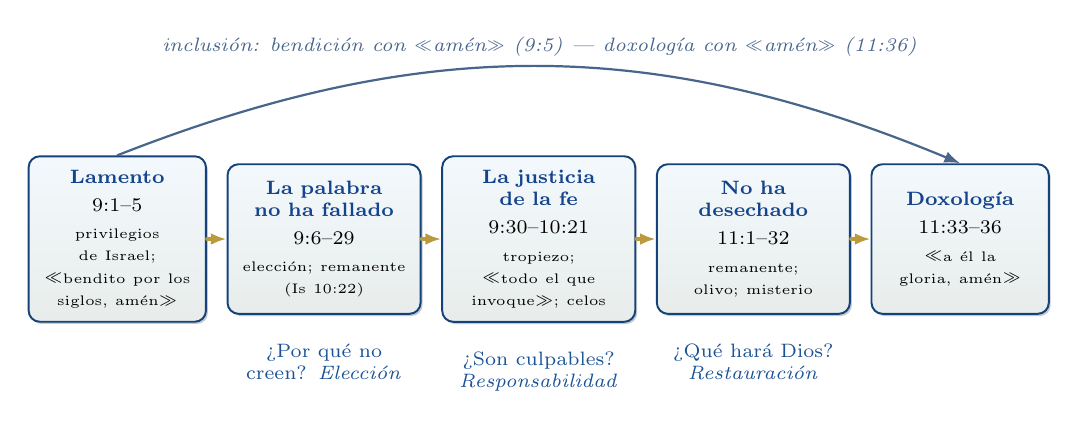
\begin{tikzpicture}[node distance=0.25cm]
\node[caja,text width=1.9cm,align=center,minimum height=1.9cm] (a) {\textbf{\textcolor{ladrillo}{Lamento}}\\[2pt]9:1--5\\[2pt]{\tiny privilegios de Israel; «bendito por los siglos, amén»}};
\node[caja,text width=2.1cm,align=center,minimum height=1.9cm,right=of a] (b) {\textbf{\textcolor{ladrillo}{La palabra no ha fallado}}\\[2pt]9:6--29\\[2pt]{\tiny elección; remanente (Is 10:22)}};
\node[caja,text width=2.1cm,align=center,minimum height=1.9cm,right=of b] (c) {\textbf{\textcolor{ladrillo}{La justicia de la fe}}\\[2pt]9:30--10:21\\[2pt]{\tiny tropiezo; «todo el que invoque»; celos}};
\node[caja,text width=2.1cm,align=center,minimum height=1.9cm,right=of c] (d) {\textbf{\textcolor{ladrillo}{No ha desechado}}\\[2pt]11:1--32\\[2pt]{\tiny remanente; olivo; misterio}};
\node[caja,text width=1.9cm,align=center,minimum height=1.9cm,right=of d,fill=oro!25] (e) {\textbf{\textcolor{ladrillo}{Doxología}}\\[2pt]11:33--36\\[2pt]{\tiny «a él la gloria, amén»}};
\foreach \u/\v in {a/b,b/c,c/d,d/e}{\draw[-{Latex[length=2mm]},oro!90!ladrillo,line width=1.2pt] (\u) -- (\v);}
\draw[sepia,line width=0.8pt,-{Latex[length=2mm]}] (a.north) to[bend left=22] node[midway,above,font=\scriptsize\itshape]{inclusión: bendición con «amén» (9:5) — doxología con «amén» (11:36)} (e.north);
\node[below=0.25cm of b,font=\scriptsize,text=cafe,text width=2.3cm,align=center] {¿Por qué no creen? \emph{Elección}};
\node[below=0.25cm of c,font=\scriptsize,text=cafe,text width=2.3cm,align=center] {¿Son culpables? \emph{Responsabilidad}};
\node[below=0.25cm of d,font=\scriptsize,text=cafe,text width=2.3cm,align=center] {¿Qué hará Dios? \emph{Restauración}};
\end{tikzpicture}\par\vspace{6pt}
\notafig{Elaboración propia: estructura de Ro 9--11.}\vspace{4pt}
\begin{clave}Ro 9:6 («no todos los de Israel son Israel») pide ser leído junto a Ro 11:26 («todo Israel será salvo»): por separado, cada uno es medio argumento.\end{clave}
\end{frame}

\begin{frame}{Diatriba y argumento}
\begin{columns}[T,onlytextwidth]
\begin{column}{0.42\textwidth}\small\RaggedRight
\textbf{\textcolor{cafe}{\grc{μὴ γένοιτο}: «¡de ningún modo!»}}\par\smallskip
Fórmula de la diatriba (Stowers, 1981); diez veces en Romanos (conteo propio).
\begin{itemize}
\item \grc{μὴ ἀπώσατο ὁ θεὸς τὸν λαὸν αὐτοῦ;} (11:1)
\item \grc{μὴ ἔπταισαν ἵνα πέσωσιν;} (11:11)
\end{itemize}
\grc{μή} anticipa respuesta negativa.\par\smallskip
Cambio de interlocutor: Israel en 3.ª persona (11:1--12) → «a vosotros, gentiles» (11:13) → «tú, olivo silvestre» (11:17).
\end{column}
\begin{column}{0.56\textwidth}
\centering
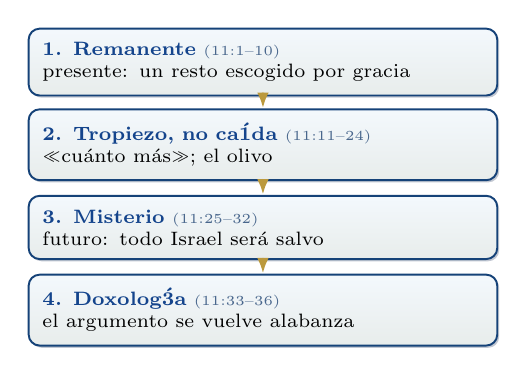
\begin{tikzpicture}[y=-1.05cm]
\foreach \i/\t/\r/\d in {0/{1. Remanente}/{11:1--10}/{presente: un resto escogido por gracia},
                        1/{2. Tropiezo, no caída}/{11:11--24}/{«cuánto más»; el olivo},
                        2/{3. Misterio}/{11:25--32}/{futuro: todo Israel será salvo},
                        3/{4. Doxología}/{11:33--36}/{el argumento se vuelve alabanza}}{
  \node[caja,text width=5.6cm,minimum height=0.8cm] (s\i) at (0,\i) {\textbf{\textcolor{ladrillo}{\t}} {\tiny\color{sepia}(\r)}\\{\scriptsize \d}};}
\foreach \a/\b in {0/1,1/2,2/3}{\draw[-{Latex[length=2mm]},oro!90!ladrillo,line width=1.2pt] (s\a) -- (s\b);}
\end{tikzpicture}\elabpropia
\end{column}
\end{columns}
\end{frame}

\begin{frame}{Las citas del AT en Ro 11}
\centering\scriptsize\renewcommand{\arraystretch}{1.05}
\begin{tabular}{>{\RaggedRight\arraybackslash}p{2.7cm}>{\RaggedRight\arraybackslash}p{2.8cm}>{\RaggedRight\arraybackslash}p{2.4cm}>{\RaggedRight\arraybackslash}p{3.6cm}}
\toprule
\color{ladrillo}\bfseries Ro 11 / fuente & \color{ladrillo}\bfseries TM & \color{ladrillo}\bfseries LXX & \color{ladrillo}\bfseries Pablo\\\midrule
11:4; 1~R 19:18 & «Dejaré (\heb{וְהִשְׁאַרְתִּי}) siete mil» & «Dejarás siete mil» & \grc{κατέλιπον ἐμαυτῷ}: más cerca del TM; «para mí»\\
11:8; Dt 29:4 [29:3] + Is 29:10 & «no os dio corazón»; \heb{רוּחַ תַּרְדֵּמָה} & \grc{πνεῦμα κατανύξεως} & Funde dos textos: «les dio ojos para no ver»\\
11:9--10; Sal 69:22--23 [LXX 68:23--24] & «Sea su mesa un lazo» & \grc{εἰς παγίδα\ldots} & Sigue la LXX; añade \grc{εἰς θήραν}\\
11:26--27; Is 59:20--21; 27:9 & «vendrá \emph{a} Sion» & «\emph{por causa de} Sion» & «\emph{de} Sion»; Is 27:9 LXX; eco de Jer 31:33--34\\
11:34; Is 40:13 & «¿quién midió el espíritu de YHWH?» & \grc{τίς ἔγνω νοῦν κυρίου;} & LXX casi literal\\
11:35; Job 41:11 [41:3] & «¿quién se me adelantó?» & otra lectura & Sigue el sentido del TM\\
\bottomrule
\end{tabular}\par
{\fontsize{5}{6}\selectfont\color{sepia}\hfill\textit{Nota.} Elaboración propia a partir de BHS, LXX (Rahlfs-Hanhart) y NA28.\par}
\begin{notalam}[Precisión textual: \grc{τῇ Βάαλ} (11:4)]
Artículo femenino para un nombre masculino: se leía \heb{בֹּשֶׁת} (\emph{bóshet}), «vergüenza», en griego \grc{αἰσχύνη}, femenino. Pablo conocía la LXX y el hebreo (Stanley, 1992; Wagner, 2002).
\end{notalam}
\end{frame}

\begin{frame}{Las metáforas}
\begin{columns}[T,onlytextwidth]
\begin{column}{0.32\textwidth}\small\RaggedRight
\textbf{\textcolor{ladrillo}{Primicias y masa}} (11:16a)\par\smallskip
Nm 15:20: \heb{רֵאשִׁית עֲרִסֹתֵכֶם}; LXX \grc{ἀπαρχὴν φυράματος}. La porción ofrecida santifica la masa. Tratado \emph{Jalá} de la Mishná.
\end{column}
\begin{column}{0.33\textwidth}\small\RaggedRight
\textbf{\textcolor{ladrillo}{Raíz y ramas}} (11:16b)\par\smallskip
«Si la raíz es santa, también las ramas». La raíz: los padres (11:28), según la mayoría de los comentaristas (Moo, 1996).
\end{column}
\begin{column}{0.32\textwidth}\small\RaggedRight
\textbf{\textcolor{ladrillo}{El olivo}} (11:17--24)\par\smallskip
\heb{זַיִת רַעֲנָן}, «olivo verde», nombre de Judá (Jer 11:16); «su esplendor como el olivo» (Os 14:6 [14:7]); Sal 52:8 [52:10].
\end{column}
\end{columns}\vspace{6pt}
\centering
\begin{tikzpicture}[node distance=0.3cm and 0.35cm]
\node[bloqueoro,text width=2.0cm] (p1) {Primicia\\{\tiny\grc{ἀπαρχή}}};
\node[bloque,text width=1.8cm,right=1.0cm of p1] (t1) {Toda la masa};
\node[bloqueoro,text width=2.0cm,right=0.9cm of t1] (p2) {Raíz: los padres\\{\tiny 11:16, 28}};
\node[bloque,text width=1.8cm,right=1.0cm of p2] (t2) {Las ramas};
\draw[flecha] (p1)--node[above,etiq]{santifica}(t1);
\draw[flecha] (p2)--node[above,etiq]{santifica}(t2);
\node[bloqueazul,text width=8.6cm,below=0.4cm of $(t1.south)!0.5!(p2.south)$] (o) {Un único olivo: ramas naturales (\grc{κατὰ φύσιν}) y silvestres injertadas; a unos y otros los sostiene la fe (11:20, 23--24)};
\draw[flecha] (t1.south) -- (o.north -| t1.south);
\draw[flecha] (t2.south) -- (o.north -| t2.south);
\end{tikzpicture}\elabpropia
\end{frame}

\begin{frame}{La doxología en quiasmo}
\begin{columns}[c,onlytextwidth]
\begin{column}{0.50\textwidth}
\begin{cita}[fontupper=\scriptsize\itshape]¡Oh profundidad de las riquezas, y de la sabiduría y del conocimiento de Dios! [\ldots] ¿Quién conoció la mente del Señor? ¿O quién fue su consejero? ¿O quién le dio a él primero? [\ldots] Porque de él, por él y para él son todas las cosas.\fuente{(Ro 11:33--36)}\end{cita}
\scriptsize Is 40:13 (consuelo del exilio) y Job 41:11 [41:3]; \grc{ἀνεξιχνίαστοι}, cf. Job 5:9; 9:10 LXX.
\end{column}
\begin{column}{0.47\textwidth}
\centering
\begin{tikzpicture}[y=-0.62cm]
\foreach \i/\t/\x in {0/{a. riqueza}/0,1/{b. sabiduría}/0.5,2/{c. conocimiento}/1.0,3/{c'. ¿quién conoció la mente?}/1.0,4/{b'. ¿quién fue su consejero?}/0.5,5/{a'. ¿quién le dio primero?}/0}{
  \node[caja,anchor=west,inner sep=3pt] at (\x,\i) {\t};}
\node[font=\tiny,text=sepia,anchor=west] at (4.6,1) {v.\,33};
\node[font=\tiny,text=sepia,anchor=west] at (4.6,4) {vv.\,34--35};
\node[caja,fill=oro!25,anchor=west] at (0,6.4) {\grc{ἐξ αὐτοῦ καὶ δι᾿ αὐτοῦ καὶ εἰς αὐτόν} (v.\,36)};
\end{tikzpicture}\par
{\fontsize{5}{6}\selectfont\color{sepia}\hfill\textit{Nota.} Elaboración propia a partir de Cranfield (1979) y Moo (1996).\par}
\end{column}
\end{columns}
\end{frame}

% ===================================================
\section{Filología}
\begin{frame}{Ro 11:25--27 en griego}
\begin{cita}[fontupper=\upshape\small]\grc{Οὐ γὰρ θέλω ὑμᾶς ἀγνοεῖν, ἀδελφοί, τὸ μυστήριον τοῦτο, ἵνα μὴ ἦτε [παρ᾿] ἑαυτοῖς φρόνιμοι, ὅτι πώρωσις ἀπὸ μέρους τῷ Ἰσραὴλ γέγονεν ἄχρι οὗ τὸ πλήρωμα τῶν ἐθνῶν εἰσέλθῃ καὶ οὕτως πᾶς Ἰσραὴλ σωθήσεται, καθὼς γέγραπται· ἥξει ἐκ Σιὼν ὁ ῥυόμενος, ἀποστρέψει ἀσεβείας ἀπὸ Ἰακώβ. καὶ αὕτη αὐτοῖς ἡ παρ᾿ ἐμοῦ διαθήκη, ὅταν ἀφέλωμαι τὰς ἁμαρτίας αὐτῶν.}\end{cita}
\begin{cita}[fontupper=\scriptsize\itshape]No quiero, hermanos, que ignoréis este misterio, para que no seáis sabios en vuestra propia opinión: que un endurecimiento en parte le ha sobrevenido a Israel hasta que haya entrado la plenitud de las naciones; y así todo Israel será salvo, como está escrito: «Vendrá de Sion el Libertador, apartará de Jacob las impiedades. Y este será mi pacto con ellos, cuando yo quite sus pecados».\fuente{(Ro 11:25--27, NA28; trad. propia)}\end{cita}
\begin{notalam}[Precisión textual en Ro 11]
Variantes que no alteran el sentido: 11:6 (adición bizantina, ausente en NA28); 11:17 («de la raíz \emph{y} de la grosura»; NA28 sigue la lectura más difícil); 11:25 (\grc{παρ᾿}/\grc{ἐν} \grc{ἑαυτοῖς}, igual sentido); 11:31 (segundo \grc{νῦν} entre corchetes; véase «Pasaje por pasaje»).
\end{notalam}
\end{frame}

\begin{frame}{Elección y remanente}
\begin{columns}[T,onlytextwidth]
\begin{column}{0.46\textwidth}\small\RaggedRight
\begin{itemize}
\item \grc{ἀπώσατο} (11:1): eco de \grc{οὐκ ἀπώσεται κύριος τὸν λαὸν αὐτοῦ} (1~S 12:22; Sal 94:14 [LXX 93:14]).
\item \heb{כִּי לֹא־יִטֹּשׁ יְהוָה אֶת־עַמּוֹ}: «YHWH no desamparará a su pueblo» (1~S 12:22; Estudio 3).
\item \grc{προέγνω} (11:2): «conoció» = eligió (Am 3:2). La elección precede a la incredulidad.
\end{itemize}
\end{column}
\begin{column}{0.52\textwidth}
\centering
\begin{tikzpicture}[y=-1.15cm]
\node[caja,text width=4.6cm,align=center] (a) at (0,0) {\textbf{Gn 45:7}: \heb{שְׁאֵרִית} (José; Est. 1)};
\node[caja,text width=4.6cm,align=center] (b) at (0,1) {\textbf{1~R 19:18}: siete mil (reino del norte; Est. 5)};
\node[caja,text width=4.6cm,align=center] (c) at (0,2) {\textbf{Is 10:21}: \heb{שְׁאָר יָשׁוּב}, «un resto volverá»};
\node[caja,text width=4.6cm,align=center,fill=oro!25] (d) at (0,3) {\textbf{Ro 11:5}: \grc{λεῖμμα κατ᾿ ἐκλογὴν χάριτος}};
\foreach \u/\v in {a/b,b/c,c/d}{\draw[-{Latex[length=2mm]},oro!90!ladrillo,line width=1.2pt] (\u) -- (\v);}
\end{tikzpicture}\elabpropia\smallskip
{\scriptsize\itshape\color{sepia}\grc{γέγονεν}, perfecto: un remanente que existe hoy y mantiene abierta la historia.}
\end{column}
\end{columns}
\end{frame}

\begin{frame}{Endurecimiento, tropiezo y celos}
\begin{columns}[T,onlytextwidth]
\begin{column}{0.49\textwidth}\small\RaggedRight
\textbf{\textcolor{cafe}{\grc{πώρωσις}} (11:7, 25)}: de \grc{πῶρος}, callo óseo, piedra porosa: insensibilidad. Velo «hasta el día de hoy» (2~Co 3:14--16).\par\smallskip
\textbf{\textcolor{cafe}{\grc{πνεῦμα κατανύξεως}} (11:8)}: Is 29:10 \heb{רוּחַ תַּרְדֵּמָה}, el «sueño profundo» de Gn 2:21 y 15:12.\par\smallskip
\textbf{\textcolor{cafe}{\grc{ἔπταισαν ἵνα πέσωσιν;}} (11:11)}: tropezar (\grc{πταίω}) no es caer (\grc{πίπτω}). \grc{παράπτωμα}: «paso en falso».
\end{column}
\begin{column}{0.49\textwidth}
\centering{\heb{וַאֲנִי אַקְנִיאֵם בְּלֹא־עָם}}\par\smallskip
\begin{cita}[fontupper=\scriptsize\itshape]Yo también los provocaré a celos con lo que no es pueblo.\fuente{(Dt 32:21; LXX \grc{παραζηλώσω})}\end{cita}
\begin{cita}[fontupper=\scriptsize\itshape]Por si de algún modo provoco a celos a los de mi carne, y salvo a algunos de ellos.\fuente{(Ro 11:14)}\end{cita}
\scriptsize La misión entre los gentiles revierte sobre Israel (Estudio 2).
\end{column}
\end{columns}
\end{frame}

\begin{frame}{Plenitud y aceptación}
\begin{columns}[T,onlytextwidth]
\begin{column}{0.49\textwidth}
\begin{cita}[fontupper=\scriptsize\itshape]Si su transgresión es la riqueza del mundo, y su disminución la riqueza de las naciones, ¡cuánto más su plenitud!\fuente{(Ro 11:12)}\end{cita}
\end{column}
\begin{column}{0.49\textwidth}
\begin{cita}[fontupper=\scriptsize\itshape]Si su exclusión es la reconciliación del mundo, ¿qué será su aceptación sino vida de entre los muertos?\fuente{(Ro 11:15)}\end{cita}
\end{column}
\end{columns}\vspace{4pt}
\centering
\begin{tikzpicture}[x=3.0cm,y=1.05cm]
\node[etiq,font=\scriptsize\bfseries,text=ladrillo] at (0,1.0) {Lo menor (ya ocurrió)};
\node[etiq,font=\scriptsize\bfseries,text=ladrillo] at (2.35,1.0) {Lo mayor (\grc{πόσῳ μᾶλλον})};
\node[bloque,text width=2.3cm] (a1) at (0,0) {\grc{παράπτωμα}, \grc{ἥττημα}\\{\tiny transgresión, disminución}};
\node[bloque,text width=1.9cm] (b1) at (1.1,0) {riqueza del mundo};
\node[bloqueoro,text width=2.3cm] (c1) at (2.35,0) {\grc{πλήρωμα αὐτῶν}\\{\tiny ¡cuánto más! (11:12)}};
\node[bloque,text width=2.3cm] (a2) at (0,-1.15) {\grc{ἀποβολή}\\{\tiny exclusión}};
\node[bloque,text width=1.9cm] (b2) at (1.1,-1.15) {reconciliación del mundo};
\node[bloqueazul,text width=2.3cm] (c2) at (2.35,-1.15) {\grc{πρόσλημψις}\\{\tiny\mdseries «vida de entre los muertos» (11:15)}};
\draw[flecha] (a1)--(b1); \draw[flecha] (b1)--(c1); \draw[flecha] (a2)--(b2); \draw[flecha] (b2)--(c2);
\end{tikzpicture}\elabpropia
\end{frame}

\begin{frame}{Plenitud y aceptación: el vocabulario}
\begin{columns}[T,onlytextwidth]
\begin{column}{0.48\textwidth}\small\RaggedRight
\begin{itemize}
\item \grc{ἥττημα}: «disminución», «derrota».
\item \grc{πλήρωμα αὐτῶν} (11:12) // \grc{πλήρωμα τῶν ἐθνῶν} (11:25): plenitud de Israel y de las naciones, en paralelo.
\item \grc{ἀποβολή}: exclusión (temporal) por parte de Dios.
\item \grc{πρόσλημψις}: «acogida»; hápax del NT.
\item \grc{ζωὴ ἐκ νεκρῶν}: resurrección o bendición inmensa; trasfondo de Ez 37:11--14 (Estudio 5).
\item \grc{ἀπαρχή}/\grc{φύραμα} (11:16): \heb{רֵאשִׁית} y la masa.
\end{itemize}
\end{column}
\begin{column}{0.48\textwidth}
\begin{notalam}[Precisión: «plenitud de las naciones» y Gn 48:19]
Gn 48:19 llama a la descendencia de Efraín \heb{מְלֹא־הַגּוֹיִם}, «plenitud de naciones». La LXX lo traduce \grc{πλῆθος ἐθνῶν}, no \grc{πλήρωμα}, y Pablo no cita ese texto. El paralelo que el propio Pablo establece está dentro de Ro 11: la plenitud de Israel (11:12) y la de las naciones (11:25).
\end{notalam}
\begin{clave}\grc{πλήρωμα} se opone a \grc{λεῖμμα}: la plenitud es más que el remanente.\end{clave}
\end{column}
\end{columns}
\end{frame}

\begin{frame}{El vocabulario del olivo}
\begin{columns}[T,onlytextwidth]
\begin{column}{0.49\textwidth}\small\RaggedRight
\begin{itemize}
\item \grc{ἀγριέλαιος}: olivo silvestre, acebuche.
\item \grc{καλλιέλαιος}: olivo cultivado, «hermoso».
\item \grc{ἐγκεντρίζω}: injertar por incisión; 6 veces en 11:17--24 (conteo propio).
\item \grc{ἐξεκλάσθησαν}: «fueron desgajadas».
\item \grc{συγκοινωνὸς τῆς ῥίζης τῆς πιότητος}: copartícipe de la savia de la raíz.
\item \grc{χρηστότης} y \grc{ἀποτομία} (11:22): bondad y «corte tajante».
\end{itemize}
\end{column}
\begin{column}{0.49\textwidth}
\centering
\begin{tikzpicture}[node distance=0.25cm and 0.3cm]
\node[bloque,text width=2.1cm] (h1) {Púa cultivada};
\node[bloque,text width=2.1cm,below=of h1] (h2) {Patrón silvestre};
\draw[flecha] (h1)--(h2);
\node[etiq,above=0.12cm of h1,font=\tiny\bfseries,text=ladrillo] {Lo habitual};
\node[bloqueoro,text width=2.1cm,right=0.6cm of h1] (p1) {Rama silvestre\\{\tiny\grc{ἀγριέλαιος}}};
\node[bloqueoro,text width=2.1cm,below=of p1] (p2) {Olivo cultivado\\{\tiny\grc{καλλιέλαιος}}};
\draw[flecha] (p1)--(p2);
\node[etiq,above=0.12cm of p1,font=\tiny\bfseries,text=ladrillo] {Ro 11:24: \grc{παρὰ φύσιν}};
\end{tikzpicture}\elabpropia
\begin{notalam}[¿Sabía Pablo injertar?]
Pablo describe lo inverso de lo habitual y lo admite: «contra la naturaleza» (11:24). Columela (\emph{De re rustica} 5.9.16) menciona una rama de acebuche insertada en olivos viejos para revitalizarlos (Baxter y Ziesler, 1985). Sigue abierto si Pablo alude a esa práctica o invierte la habitual para subrayar la gracia.
\end{notalam}
\end{column}
\end{columns}
\end{frame}

\begin{frame}{«Para que no seáis sabios en vuestra opinión»}
\begin{columns}[T,onlytextwidth]
\begin{column}{0.52\textwidth}\scriptsize\RaggedRight
\grc{ἵνα μὴ ἦτε [παρ᾿] ἑαυτοῖς φρόνιμοι} (Ro 11:25)\par\smallskip
\begin{itemize}
\item Eco de Pr 3:7 LXX: \grc{μὴ ἴσθι φρόνιμος παρὰ σεαυτῷ}; hebreo \heb{אַל־תְּהִי חָכָם בְּעֵינֶיךָ}, «no seas sabio a tus propios ojos».
\item Pablo lo repite en Ro 12:16.
\item RVR1960: «para que no seáis \textbf{arrogantes} en cuanto a vosotros mismos»; NVI: «presuntuosos».
\end{itemize}
\end{column}
\begin{column}{0.46\textwidth}\scriptsize\RaggedRight
\textbf{\textcolor{cafe}{\grc{μυστήριον}}}: 28 veces en el NT, 21 en Pablo (conteo propio).\par\smallskip
Agustín: \emph{Novum in Vetere latet, Vetus in Novo patet} (\emph{Quaest. in Hept.} 2.73).\par\medskip
\begin{tcolorbox}[colback=piedra,colframe=ladrillo,boxrule=0.8pt,arc=2pt,fontupper=\scriptsize]
Desconocer el plan de Dios con Israel tiene consecuencias: \textbf{da alimento a la soberbia} gentil (11:18, 20).
\end{tcolorbox}
\end{column}
\end{columns}
\end{frame}

\begin{frame}{Misterio, «en parte», «hasta que»}
\begin{columns}[T,onlytextwidth]
\begin{column}{0.33\textwidth}\small\RaggedRight
\textbf{\textcolor{ladrillo}{\grc{μυστήριον}}}\par\smallskip
Designio antes oculto, ahora revelado (Ro 16:25--26). Trasfondo: arameo \heb{רָז} (\emph{raz}) de Dn 2:18--30; Qumrán (1QpHab 7). La novedad está en \destacar{el orden}, no en la restauración.
\end{column}
\begin{column}{0.31\textwidth}\small\RaggedRight
\textbf{\textcolor{ladrillo}{\grc{ἀπὸ μέρους}}}\par\smallskip
«En parte»: endurecimiento parcial, o sobre una parte de Israel. En ambos casos, el remanente queda fuera (11:5, 7).
\end{column}
\begin{column}{0.33\textwidth}\small\RaggedRight
\textbf{\textcolor{ladrillo}{\grc{ἄχρι οὗ}}}\par\smallskip
«Hasta que» + subjuntivo: término de una situación.
\begin{itemize}
\item Lc 21:24: Jerusalén hollada \grc{ἄχρι οὗ} se cumplan los tiempos de los gentiles.
\item 1~Co 11:26; 15:25.
\end{itemize}
\grc{εἰσέλθῃ}: verbo de «entrar en el reino».
\end{column}
\end{columns}\vspace{4pt}
\centering
\begin{tikzpicture}[x=1cm,etiq/.append style={font=\scriptsize}]
\fill[oro!70] (0,0.04) rectangle (6.4,0.44);
\fill[ladrillo!70] (0,-0.44) rectangle (6.4,-0.04);
\node[etiq,anchor=east] at (-0.15,0.24) {remanente creyente (11:5)};
\node[etiq,anchor=east] at (-0.15,-0.24) {mayoría: \grc{πώρωσις ἀπὸ μέρους}};
\draw[oro!90!ladrillo,line width=1.4pt] (6.4,-0.5) -- (6.4,0.5);
\node[etiq,above] at (6.4,0.5) {\grc{ἄχρι οὗ}: entra la plenitud};
\node[bloqueazul,anchor=west,text width=2.6cm] (f) at (7.0,0) {y así todo Israel será salvo (11:26)};
\draw[flecha] (6.45,0) -- (f.west);
\end{tikzpicture}\elabpropia
\end{frame}

\begin{frame}{«Y así»: tres lecturas}
\centering\footnotesize\renewcommand{\arraystretch}{1.3}
\begin{tabular}{>{\RaggedRight\arraybackslash}p{2.3cm}>{\RaggedRight\arraybackslash}p{4.3cm}>{\RaggedRight\arraybackslash}p{4.4cm}}
\toprule
\color{ladrillo}\bfseries \grc{καὶ οὕτως} & \color{ladrillo}\bfseries Sentido & \color{ladrillo}\bfseries Defensores\\\midrule
Modal: «y de esta manera» & Mediante el proceso descrito: endurecimiento, entrada de las naciones, celos & Cranfield (1979); Moo (1996); Schreiner (1998); Fitzmyer (1993)\\
Temporal: «y entonces» & Después de la entrada de las naciones & Van der Horst (2000); RVR: «y luego»\\
Correlativa: «así, como está escrito» & \grc{οὕτως} anticipa \grc{καθὼς γέγραπται} & Matiz señalado por Dunn (1988)\\
\bottomrule
\end{tabular}\par
\elabpropia
\vspace{4pt}
\begin{clave}
Punto común: la salvación de «todo Israel» \textbf{viene después} del endurecimiento parcial y de la entrada de la plenitud de las naciones. Un versículo antes (11:25), «Israel» y «las naciones» aparecen como grupos distintos.
\end{clave}
\end{frame}

\begin{frame}{\grc{πᾶς Ἰσραήλ}: «todo Israel»}
\begin{columns}[T,onlytextwidth]
\begin{column}{0.49\textwidth}\small
\textbf{\textcolor{cafe}{Uso colectivo en el AT}} (\heb{כָּל־יִשְׂרָאֵל})
\begin{itemize}
\item 1~S 25:1: todo Israel llora a Samuel.
\item 1~R 12:1: todo Israel en Siquem (Est. 4).
\item 2~Cr 12:1: «todo Israel» = el reino de Judá.
\item Dn 9:11: «todo Israel traspasó tu ley».
\item Neh 12:47: todo Israel sostiene a los cantores.
\end{itemize}
\scriptsize El conjunto del pueblo: ni cada individuo ni extranjeros.
\end{column}
\begin{column}{0.49\textwidth}\small
\textbf{\textcolor{cafe}{Mishná, Sanedrín 10:1}}\par\smallskip
\centering{\heb{כל ישראל יש להם חלק לעולם הבא}}\par\smallskip
\raggedright «Todo Israel tiene parte en el mundo venidero» \ldots{} \textbf{y a continuación enumera quiénes no la tienen}.\par\medskip
\grc{Ἰσραήλ}: 11 veces en Ro 9--11, siempre el pueblo étnico (9:6b: un Israel \emph{dentro} de Israel).\par\smallskip
\grc{σωθήσεται}: futuro pasivo; obra de Dios; salvación por la fe (10:9--13).
\end{column}
\end{columns}
\end{frame}

\begin{frame}{Is 59:20: TM, LXX y Pablo}
\centering\scriptsize\renewcommand{\arraystretch}{1.35}
\begin{tabular}{>{\RaggedRight\arraybackslash}p{1.6cm}>{\RaggedRight\arraybackslash}p{4.3cm}>{\RaggedRight\arraybackslash}p{5.2cm}}
\toprule
\color{ladrillo}\bfseries Versión & \color{ladrillo}\bfseries Texto & \color{ladrillo}\bfseries Traducción\\\midrule
TM & \heb{וּבָא לְצִיּוֹן גּוֹאֵל וּלְשָׁבֵי פֶשַׁע בְּיַעֲקֹב} & «Vendrá \textbf{a} Sion un Redentor, y a los que se vuelven de la rebelión en Jacob»\\
LXX & \grc{ἥξει ἕνεκεν Σιων ὁ ῥυόμενος καὶ ἀποστρέψει ἀσεβείας ἀπὸ Ιακωβ} & «Vendrá \textbf{por causa de} Sion el que libra, y apartará las impiedades de Jacob»\\
Pablo & \grc{ἥξει ἐκ Σιὼν ὁ ῥυόμενος, ἀποστρέψει ἀσεβείας ἀπὸ Ἰακώβ} & «Vendrá \textbf{de} Sion el Libertador, apartará de Jacob las impiedades»\\
\bottomrule
\end{tabular}\par
\elabpropia\vspace{3pt}
\begin{minipage}{0.95\linewidth}\scriptsize
\textbf{\grc{ἐκ Σιών}}: ecos de Sal 14:7 e Is 2:3; la Sion celestial y la segunda venida (Cranfield, 1979; Moo, 1996; cf. 1~Ts 1:10, \grc{τὸν ῥυόμενον}), o la misión desde Jerusalén (Wright, 2013).\par\smallskip
\textbf{Pacto}: Is 59:21 + 27:9 LXX («cuando yo quite sus pecados») evocan Jer 31:33--34 [31:32--33]: el nuevo pacto con Israel y Judá (Estudio 5).
\end{minipage}
\end{frame}

\begin{frame}{El Redentor de Sion}
\fotolado{panel_is59.jpg}{Elaboración propia: Is 59:20--21a en texto hebreo consonántico (BHS).}
\begin{columns}[c,onlytextwidth]
\begin{column}{0.57\textwidth}
\centering{\large\heb{וּבָא לְצִיּוֹן גּוֹאֵל}}\par\smallskip
\begin{cita}Y vendrá a Sion el Redentor, y a los que se vuelven de la rebelión en Jacob, dice YHWH. Y en cuanto a mí, este es mi pacto con ellos.\fuente{(Is 59:20--21)}\end{cita}
\scriptsize
\begin{itemize}
\item \heb{גּוֹאֵל} (\emph{go'el}): el pariente que rescata (Rut; Is 41:14).
\item TM: primero el arrepentimiento. LXX y Pablo: el acento en la acción del Libertador.
\item Estos versículos abren la oración diaria \emph{U-va le-Tsiyyón} de la liturgia judía.
\end{itemize}
\end{column}
\begin{column}{0.41\textwidth}\end{column}
\end{columns}
\end{frame}

\begin{frame}{«Y así todo Israel»}
\fotolado{panel_ro26.jpg}{Elaboración propia: Ro 11:25b--26 en escritura uncial (texto NA28).}
\begin{columns}[c,onlytextwidth]
\begin{column}{0.57\textwidth}
\begin{cita}Un endurecimiento en parte le ha sobrevenido a Israel hasta que haya entrado la plenitud de las naciones; y así todo Israel será salvo.\fuente{(Ro 11:25b--26a)}\end{cita}
\scriptsize
\begin{itemize}
\item \grc{ἀμεταμέλητα} (11:29): «sin arrepentimiento»; Nm 23:19.
\item \grc{ἐχθροί … ἀγαπητοί} (11:28): enemigos y amados \emph{a la vez}.
\item \grc{συνέκλεισεν} (11:32): «encerró juntos», como la red (Lc 5:6; Gá 3:22).
\item \grc{βάθος} (11:33): Pablo termina con «profundidad».
\end{itemize}
\end{column}
\begin{column}{0.41\textwidth}\end{column}
\end{columns}
\end{frame}

% ===================================================
\section{Teología}
\begin{frame}{La fidelidad de Dios}
\begin{columns}[T,onlytextwidth]
\begin{column}{0.49\textwidth}\small\RaggedRight
Si Dios abandonó a Israel, ¿qué valor tiene Ro 8:39, «nada nos podrá separar»?\par\medskip
\destacar{Ro 9:6}: «no es que la palabra de Dios haya fallado».\par\medskip
Ro 11 cierra la demostración: elección anterior a la historia (\grc{προέγνω}) e irrevocable (\grc{ἀμεταμέλητα}).
\end{column}
\begin{column}{0.49\textwidth}
\centering
{\small\textbf{\textcolor{ladrillo}{Los límites del endurecimiento}}}\par\smallskip
\begin{tikzpicture}
\node[bloqueazul,text width=1.9cm] (c) at (0,0) {\grc{πώρωσις}\\{\tiny\mdseries 11:7, 25}};
\node[bloque,text width=1.9cm] (p) at (-1.55,-1.65) {\textbf{Parcial}\\{\tiny\grc{ἀπὸ μέρους}: existe el remanente}};
\node[bloque,text width=1.9cm] (t) at (1.55,-1.65) {\textbf{Temporal}\\{\tiny\grc{ἄχρι οὗ}: tiene término}};
\node[bloqueoro,text width=2.4cm] (q) at (0,1.45) {\textbf{Con propósito}\\{\tiny salvación de las naciones y celos de Israel (11:11)}};
\draw[flecha] (c)--(p); \draw[flecha] (c)--(t); \draw[flecha] (c)--(q);
\end{tikzpicture}\elabpropia
\begin{clave}Razones: soberanía (9:18), ignorancia (10:4), justicia propia (10:3); temporalidad (11:26). Juicio de Dios y responsabilidad humana a la vez.\end{clave}
\end{column}
\end{columns}
\end{frame}

\begin{frame}{El olivo}
\centering
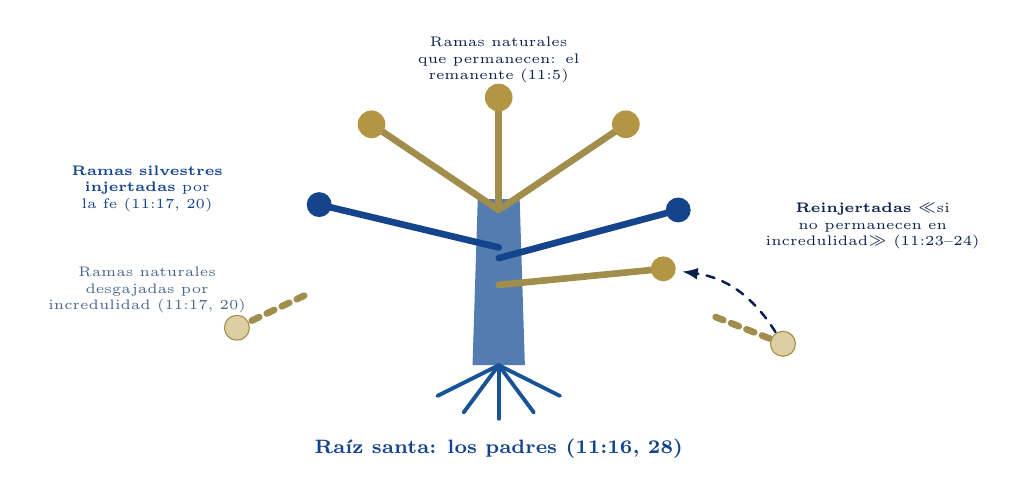
\begin{tikzpicture}[x=0.95cm,y=0.68cm]
\fill[cafe!75] (-0.35,0) -- (-0.28,3.1) -- (0.28,3.1) -- (0.35,0) -- cycle;
\foreach \a in {-55,-28,0,28,55}{\draw[cafe,line width=1.4pt] (0,0) -- ++(-90+\a:1.0);}
\node[font=\scriptsize\bfseries,text=ladrillo] at (0,-1.55) {Raíz santa: los padres (11:16, 28)};
\foreach \x/\y in {-1.7/4.5, 0/5.0, 1.7/4.5}{\draw[oro!75!cafe,line width=2.4pt] (0,2.9) -- (\x,\y); \fill[oro!85!cafe] (\x,\y) circle (5pt);}
\node[font=\tiny,text=cafeosc,text width=3.2cm,align=center] at (0,5.7) {Ramas naturales que permanecen: el remanente (11:5)};
\draw[ladrillo,line width=2.4pt] (0,2.2) -- (-2.4,3.0); \fill[ladrillo] (-2.4,3.0) circle (4.5pt);
\draw[ladrillo,line width=2.4pt] (0,2.0) -- (2.4,2.9); \fill[ladrillo] (2.4,2.9) circle (4.5pt);
\node[font=\tiny,text=ladrillo,text width=2.8cm,align=center] at (-4.7,3.3) {\textbf{Ramas silvestres injertadas} por la fe (11:17, 20)};
\draw[oro!75!cafe,line width=2.4pt,dashed] (-2.6,1.3) -- (-3.5,0.7); \fill[oro!45!piedra,draw=oro!75!cafe] (-3.5,0.7) circle (4.5pt);
\node[font=\tiny,text=sepia,text width=2.8cm,align=center] at (-4.7,1.4) {Ramas naturales desgajadas por incredulidad (11:17, 20)};
\draw[oro!75!cafe,line width=2.4pt,dashed] (2.9,0.9) -- (3.8,0.4); \fill[oro!45!piedra,draw=oro!75!cafe] (3.8,0.4) circle (4.5pt);
\draw[oro!75!cafe,line width=2.4pt] (0,1.5) -- (2.2,1.8); \fill[oro!85!cafe] (2.2,1.8) circle (4.5pt);
\draw[-{Latex[length=2mm]},cafeosc,line width=0.9pt,dashed] (3.7,0.62) to[bend right=25] (2.45,1.75);
\node[font=\tiny,text=cafeosc,text width=3.0cm,align=center] at (5.0,2.6) {\textbf{Reinjertadas} «si no permanecen en incredulidad» (11:23--24)};
\end{tikzpicture}\par\vspace{2pt}
{\scriptsize Injertados «entre» las ramas (\grc{ἐν αὐτοῖς}): \destacar{inclusión sin reemplazo}. «No sustentas tú a la raíz, sino la raíz a ti» (11:18).}\par
{\fontsize{5}{6}\selectfont\color{sepia}\raggedleft\textit{Nota.} Elaboración propia: esquema del olivo de Ro 11:16--24.\par}
\end{frame}

\begin{frame}{El misterio: la secuencia}
\centering
\begin{tikzpicture}[node distance=0.5cm]
\node[caja,text width=3.0cm,align=center,minimum height=2.0cm] (a) {\small\textbf{\textcolor{ladrillo}{Endurecimiento en parte}}\\[3pt]\grc{πώρωσις}\\\grc{ἀπὸ μέρους}\\[2pt]{\tiny remanente creyente + mayoría endurecida}};
\node[caja,text width=3.0cm,align=center,minimum height=2.0cm,right=of a] (b) {\small\textbf{\textcolor{ladrillo}{Entra la plenitud de las naciones}}\\[3pt]\grc{ἄχρι οὗ τὸ πλήρωμα}\\\grc{τῶν ἐθνῶν εἰσέλθῃ}};
\node[caja,text width=3.0cm,align=center,minimum height=2.0cm,right=of b,fill=oro!25] (c) {\small\textbf{\textcolor{ladrillo}{Y así todo Israel será salvo}}\\[3pt]\grc{καὶ οὕτως πᾶς}\\\grc{Ἰσραὴλ σωθήσεται}};
\draw[-{Latex[length=2.5mm]},oro!90!ladrillo,line width=1.4pt] (a) -- (b);
\draw[-{Latex[length=2.5mm]},oro!90!ladrillo,line width=1.4pt] (b) -- (c);
\end{tikzpicture}\par\vspace{8pt}
\begin{cita}[fontupper=\scriptsize\itshape]Vendrá de Sion el Libertador, apartará de Jacob las impiedades. Y este será mi pacto con ellos, cuando yo quite sus pecados.\fuente{(Ro 11:26b--27; Is 59:20--21; 27:9; Jer 31:33--34)}\end{cita}
{\scriptsize Los profetas: Israel restaurado y las naciones acuden (Is 2:2--4; Zac 8:23). \destacar{El misterio invierte el orden}: primero entran las naciones.}\par
{\fontsize{5}{6}\selectfont\color{sepia}\raggedleft\textit{Nota.} Elaboración propia: la secuencia de Ro 11:25--27.\par}
\end{frame}

\begin{frame}{¿Por qué tropezó Israel?}
\begin{columns}[T,onlytextwidth]
\begin{column}{0.49\textwidth}\scriptsize\RaggedRight
\textbf{\textcolor{cafe}{La piedra de tropiezo}}
\begin{itemize}
\item «Maldito por Dios es el colgado» (Dt 21:23; Gá 3:13).
\item Cristo crucificado: \grc{σκάνδαλον} para los judíos (1~Co 1:23).
\item La «piedra de tropiezo» de Is 8:14; 28:16 es el Mesías (Ro 9:32--33).
\item Se esperaba un rey que librara de Roma; llegó un siervo sufriente (Is 53).
\end{itemize}
\end{column}
\begin{column}{0.49\textwidth}\scriptsize\RaggedRight
\textbf{\textcolor{cafe}{Los gentiles también estaban endurecidos}}
\begin{itemize}
\item «Dios los \textbf{entregó}» (\grc{παρέδωκεν}): Ro 1:24, 26, 28.
\item «Sin Cristo, ajenos a los pactos, sin esperanza» (Ef 2:12).
\item Ef 4:18: «por la \textbf{dureza} de su corazón», \grc{διὰ τὴν πώρωσιν}: \textbf{la misma palabra} de Ro 11:25.
\end{itemize}
\begin{tcolorbox}[colback=piedra,colframe=ladrillo,boxrule=0.8pt,arc=2pt,fontupper=\scriptsize]
La \emph{pṓrōsis} de Israel no es peor que la de las naciones: «Dios encerró a todos» (11:32).
\end{tcolorbox}
\end{column}
\end{columns}
\end{frame}

\begin{frame}{Amados por los padres}
\fotolado{panel_jer31.jpg}{Elaboración propia: Jer 31:35a, 36 en texto hebreo consonántico (BHS).}
\begin{columns}[c,onlytextwidth]
\begin{column}{0.57\textwidth}
\begin{cita}[fontupper=\scriptsize\itshape]En cuanto al evangelio, enemigos por causa de vosotros; en cuanto a la elección, amados por causa de los padres.\fuente{(Ro 11:28)}\end{cita}
\centering{\heb{גַּם זֶרַע יִשְׂרָאֵל יִשְׁבְּתוּ מִהְיוֹת גּוֹי}}\par\smallskip
\begin{cita}[fontupper=\scriptsize\itshape]Si faltaren estas leyes delante de mí, dice YHWH, también la descendencia de Israel dejará de ser nación delante de mí todos los días.\fuente{(Jer 31:36 [31:35])}\end{cita}
\scriptsize Un mismo pacto perdona (Jer 31:31--34) y conserva al pueblo (31:35--37).
\end{column}
\begin{column}{0.41\textwidth}\end{column}
\end{columns}
\end{frame}

\begin{frame}{«Por amor de Jonatán tu padre»}
\begin{columns}[T,onlytextwidth]
\begin{column}{0.44\textwidth}\footnotesize\RaggedRight
\textbf{\textcolor{cafe}{La base: Dt 7:7--8}}\par
«No por ser vosotros más que todos los pueblos [\ldots] sino por cuanto YHWH os amó, y quiso guardar el juramento que juró a \textbf{vuestros padres}».\par\medskip
\textbf{\textcolor{cafe}{La imagen: Mefiboset}} (Estudio 4)\par
«Haré contigo misericordia (\heb{חֶסֶד}) \textbf{por amor de Jonatán tu padre}» (2~S 9:7). Lisiado, sin méritos, come siempre a la mesa del rey.
\end{column}
\begin{column}{0.53\textwidth}
\centering
\begin{tikzpicture}[node distance=0.32cm and 0.3cm]
\node[etiq,font=\tiny\bfseries,text=ladrillo] (h1) {Estudio 4};
\node[etiq,font=\tiny\bfseries,text=ladrillo,right=2.05cm of h1] (h2) {Ro 11:28--29};
\node[bloqueoro,text width=2.3cm,below=0.15cm of h1] (a1) {Pacto David--Jonatán\\{\tiny 1~S 20:14--17, 42}};
\node[bloqueoro,text width=2.3cm,below=0.15cm of h2] (a2) {Pacto con los padres\\{\tiny Gn 15; 17:7; Dt 7:8}};
\node[bloque,text width=2.3cm,below=of a1] (b1) {\heb{חֶסֶד} «por amor de Jonatán»};
\node[bloque,text width=2.3cm,below=of a2] (b2) {«Amados por causa de los padres»};
\node[bloqueazul,text width=2.3cm,below=of b1] (c1) {Mefiboset a la mesa del rey};
\node[bloqueazul,text width=2.3cm,below=of b2] (c2) {Israel: llamamiento irrevocable};
\draw[flecha] (a1)--(b1); \draw[flecha] (b1)--(c1);
\draw[flecha] (a2)--(b2); \draw[flecha] (b2)--(c2);
\draw[sepia,densely dashed] (b1)--node[above,etiq]{como}(b2);
\end{tikzpicture}\elabpropia
\end{column}
\end{columns}
\begin{notalam}[Enemigos y amados a la vez]
El hijo pródigo (Lc 15:11--32) actúa como enemigo de la casa mientras el padre lo ama y lo espera. Límite de la imagen: la parábola habla de un individuo; Ro 11:28, de un pueblo y una elección colectiva. El fundamento es el pacto, no la conducta de cada generación (Nm 23:19).
\end{notalam}
\end{frame}

\begin{frame}{Misericordia para todos}
\begin{columns}[c,onlytextwidth]
\begin{column}{0.52\textwidth}
\begin{cita}Porque Dios encerró a todos en desobediencia, para tener misericordia de todos.\fuente{(Ro 11:32)}\end{cita}
\small «Todos» (\grc{τοὺς πάντας}): los dos grupos del contexto, gentiles e Israel.\par\medskip
Nadie puede alegar mérito: unos y otros dependen de la misma misericordia.
\end{column}
\begin{column}{0.45\textwidth}
\centering
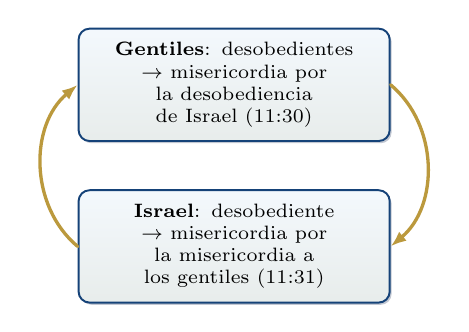
\begin{tikzpicture}[node distance=0.6cm]
\node[caja,text width=3.6cm,align=center] (g) {\textbf{Gentiles}: desobedientes $\to$ misericordia por la desobediencia de Israel (11:30)};
\node[caja,text width=3.6cm,align=center,below=of g] (i) {\textbf{Israel}: desobediente $\to$ misericordia por la misericordia a los gentiles (11:31)};
\draw[-{Latex[length=2mm]},oro!90!ladrillo,line width=1.2pt] (g.east) to[bend left=50] (i.east);
\draw[-{Latex[length=2mm]},oro!90!ladrillo,line width=1.2pt] (i.west) to[bend left=50] (g.west);
\end{tikzpicture}\elabpropia
\end{column}
\end{columns}
\end{frame}

\begin{frame}{Nación santa en Romanos 11}
\centering
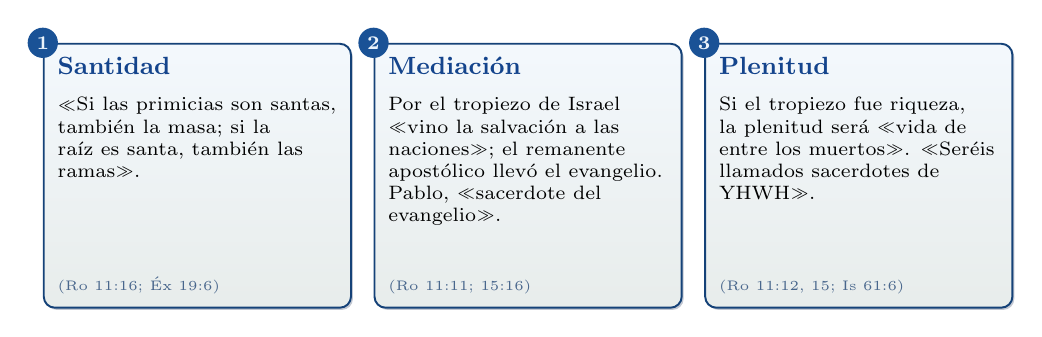
\begin{tikzpicture}
 \foreach \x/\n/\t/\d/\r in {0/1/{Santidad}/{«Si las primicias son santas, también la masa; si la raíz es santa, también las ramas».}/{Ro 11:16; Éx 19:6},
   4.2/2/{Mediación}/{Por el tropiezo de Israel «vino la salvación a las naciones»; el remanente apostólico llevó el evangelio. Pablo, «sacerdote del evangelio».}/{Ro 11:11; 15:16},
   8.4/3/{Plenitud}/{Si el tropiezo fue riqueza, la plenitud será «vida de entre los muertos». «Seréis llamados sacerdotes de YHWH».}/{Ro 11:12, 15; Is 61:6}}{
  \node[caja,anchor=north] (b\n) at (\x,0) {\parbox[t][3.0cm][t]{3.55cm}{\RaggedRight
    {\small\textbf{\textcolor{ladrillo}{\t}}}\\[5pt]\scriptsize \d\par\vfill{\tiny\color{sepia}(\r)}}};
  \node[circle,fill=cafe,text=piedra,font=\scriptsize\bfseries,inner sep=1.6pt] at (b\n.north west) {\n};}
\end{tikzpicture}\par\vspace{6pt}
{\small\itshape\color{sepia}El sacerdocio de Israel no ha sido cancelado; aguarda su forma completa.}
\elabpropia
\end{frame}

% ===================================================
\section{Pasaje por pasaje}
\newcommand{\tabpost}[6]{%
\centering\scriptsize\renewcommand{\arraystretch}{1.18}
\begin{tabular}{>{\RaggedRight\arraybackslash}p{2.3cm}>{\RaggedRight\arraybackslash}p{8.9cm}}
\toprule
\color{ladrillo}\bfseries Postura & \color{ladrillo}\bfseries Cómo lee el pasaje\\\midrule
1. Iglesia & #1\\
2. Remanente & #2\\
3. Todos & #3\\
4. Dos caminos & #4\\
5. Dos Casas & #5\\
6. Israel futuro & #6\\
\bottomrule
\end{tabular}\par
{\fontsize{5}{6}\selectfont\color{sepia}\hfill\textit{Nota.} Elaboración propia.\par}}

\begin{frame}{Seis posturas, ocho pasajes}
\begin{columns}[T,onlytextwidth]
\begin{column}{0.52\textwidth}\scriptsize
\textbf{\textcolor{cafe}{Clave de las posturas}}
\begin{itemize}
\item \textbf{1.} La iglesia (Calvino; Wright).
\item \textbf{2.} Remanente de todas las épocas (Hendriksen; Robertson; \textbf{Miguel Núñez}).
\item \textbf{3.} Todos los judíos.
\item \textbf{4.} Dos caminos (Stendahl; Gaston; Gager).
\item \textbf{5.} Dos Casas (Koniuchowsky).
\item \textbf{6.} Israel étnico futuro que reconoce al Mesías (Murray; Cranfield; Moo; Schreiner).
\end{itemize}
\end{column}
\begin{column}{0.46\textwidth}
\centering
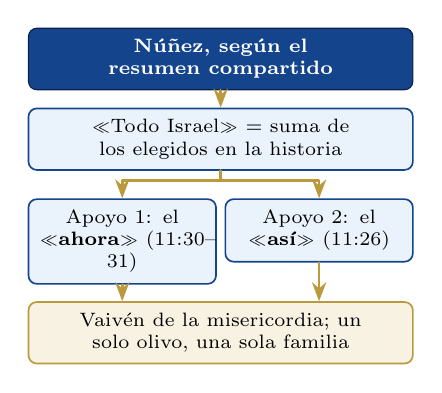
\begin{tikzpicture}[node distance=0.22cm]
\node[bloqueazul,text width=4.6cm] (n) {Núñez, según el resumen compartido};
\node[bloque,text width=4.6cm,below=of n] (a) {«Todo Israel» = suma de los elegidos en la historia};
\node[bloque,text width=2.1cm,below=0.35cm of a.south west,anchor=north west] (b) {Apoyo 1: el «\textbf{ahora}» (11:30--31)};
\node[bloque,text width=2.1cm,below=0.35cm of a.south east,anchor=north east] (c) {Apoyo 2: el «\textbf{así}» (11:26)};
\node[bloqueoro,text width=4.6cm,below=0.35cm of $(b.south)!0.5!(c.south)$] (d) {Vaivén de la misericordia; un solo olivo, una sola familia};
\draw[flecha] (n)--(a); \draw[flecha] (a.south) -- ++(0,-0.12) -| (b.north); \draw[flecha] (a.south) -- ++(0,-0.12) -| (c.north);
\draw[flecha] (b.south) -- (b.south |- d.north); \draw[flecha] (c.south) -- (c.south |- d.north);
\end{tikzpicture}\elabpropia
\begin{clave}Postura 2, con un matiz de la 1. A examen, sus dos apoyos: «ahora» y «así».\end{clave}
\end{column}
\end{columns}
\end{frame}

\begin{frame}{Pasaje 1 (11:1--6): remanente presente}
\begin{cita}[fontupper=\scriptsize\itshape]\grc{οὕτως οὖν καὶ ἐν τῷ νῦν καιρῷ λεῖμμα κατ᾿ ἐκλογὴν χάριτος γέγονεν}: «así también en el tiempo presente ha llegado a existir un remanente según la elección de la gracia».\fuente{(Ro 11:5)}\end{cita}
\tabpost{El remanente, con los gentiles, es el verdadero Israel.}%
{El remanente de hoy, sumado en la historia, es «todo Israel».}%
{«No desechó» = ningún judío fuera; pero solo «la elección» alcanzó (11:7).}%
{El remanente que Pablo muestra cree en Jesús: él mismo.}%
{Elías y los siete mil eran del norte; Pablo los usa como modelo, no como Efraín oculto.}%
{El remanente es prenda y comienzo; se opone a la «plenitud» (11:12).}
\par\vspace{2pt}\precision{el «ahora» de Pablo (\grc{νῦν καιρός}) es el tiempo \emph{del remanente}. Variante 11:1: P46 y G leen «su heredad».}
\end{frame}

\begin{frame}{Pasaje 2 (11:7--10): elegidos y endurecidos}
\begin{cita}[fontupper=\scriptsize\itshape]«La elección lo alcanzó, y los demás fueron endurecidos» \ldots{} «encorva su espalda \grc{διὰ παντός}» (\heb{תָּמִיד}, «continuamente»).\fuente{(Ro 11:7, 10; Sal 69:23)}\end{cita}
\tabpost{«Los demás» quedan fuera; lo de Israel que permanece entra en la iglesia.}%
{Cada generación se divide en elegidos y endurecidos.}%
{No explica que «los demás» no alcanzaran lo que buscaban.}%
{El endurecimiento abriría paso a los gentiles sin que Israel deba creer; Pablo lo ve como velo que se quita (2~Co 3:14--16).}%
{Sin lectura propia: habla del Israel judío de Pablo.}%
{Endurecimiento real, parcial y temporal: «continuamente» mientras dure; 11:25 le pone límite.}
\end{frame}

\begin{frame}{Pasaje 3 (11:11--12): el vaivén aparece}
\begin{cita}[fontupper=\scriptsize\itshape]Por su transgresión vino la salvación a las naciones, \textbf{para provocarlos a celos}. Y si su transgresión es riqueza para el mundo, ¡\textbf{cuánto más} su plenitud!\fuente{(Ro 11:11--12)}\end{cita}
\tabpost{La «plenitud» sería su entrada en la iglesia; pero no sería un bien \emph{mayor}.}%
{El vaivén ya opera; la plenitud es la suma de los atraídos.}%
{Plenitud = cada judío; el «cuánto más» no lo exige.}%
{Los celos buscan que Israel reciba la misma salvación (11:14).}%
{Plenitud de las tribus; pero es la plenitud de «ellos», los que tropezaron.}%
{Vaivén presente que apunta a un resultado mayor: plenitud frente a remanente.}
\par\vspace{2pt}\precision{\emph{qal va-jómer}: de lo menor (\grc{ἥττημα}) a lo mayor (\grc{πλήρωμα}).}
\end{frame}

\begin{frame}{Pasaje 4 (11:13--16): «algunos» y «vida de entre los muertos»}
\begin{cita}[fontupper=\scriptsize\itshape]Por si de algún modo provoco a celos a los de mi carne y salvo a \textbf{algunos} de ellos \ldots{} ¿qué será su aceptación sino vida de entre los muertos?\fuente{(Ro 11:14--15)}\end{cita}
\centering\scriptsize
\begin{tikzpicture}[x=2.85cm]
\foreach \i/\g/\v/\t in {0/λεῖμμα/11:5/remanente,1/τινάς/11:14/algunos,2/πλήρωμα/11:12/plenitud,3/πᾶς Ἰσραήλ/11:26/todo Israel}
  \node[caja,minimum width=2.25cm,text width=2.05cm,align=center] (n\i) at (\i,0) {\grc{\g}\\«\t» (\v)};
\draw[-{Stealth},oro,line width=1.2pt] (n0)--(n1); \draw[-{Stealth},oro,line width=1.2pt] (n1)--(n2); \draw[-{Stealth},oro,line width=1.2pt] (n2)--(n3);
\draw[decorate,decoration={brace,mirror,amplitude=4pt},cafe] ([yshift=-3pt]n0.south west)--([yshift=-3pt]n1.south east) node[midway,below=5pt]{«ya»: el presente de Pablo};
\draw[decorate,decoration={brace,mirror,amplitude=4pt},ladrillo] ([yshift=-3pt]n2.south west)--([yshift=-3pt]n3.south east) node[midway,below=5pt]{«todavía no»};
\end{tikzpicture}\elabpropia\vspace{4pt}
\raggedright\scriptsize
\textbf{2 (Núñez)}: el ministerio de Pablo prueba que el proceso es presente. \textbf{6}: es presente, pero salva a «algunos»; la «aceptación» será de otro orden (Ez 37:11--14). \textbf{3}: «algunos» la contradice.
\end{frame}

\begin{frame}{Pasaje 5 (11:17--24): un solo olivo}
\begin{cita}[fontupper=\scriptsize\itshape]¡Cuánto más estos, las ramas \textbf{naturales} (\grc{κατὰ φύσιν}), \textbf{serán injertados} en \textbf{su propio} olivo (\grc{τῇ ἰδίᾳ ἐλαίᾳ})!\fuente{(Ro 11:24)}\end{cita}
\tabpost{Un solo pueblo; las distinciones de origen se superan.}%
{Un solo olivo, una sola familia; reinjerto cada vez que un judío cree.}%
{Choca con «si no permanecen en incredulidad» (11:23).}%
{Choca con la misma condición de fe.}%
{Choca con «olivo silvestre por naturaleza»: Efraín serían ramas naturales.}%
{Un solo olivo, pero «su propio olivo»; futuro pasivo: reinjerto por venir.}
\par\vspace{2pt}\precision{con Núñez: no hay dos árboles. Aun así, el texto distingue ramas naturales y silvestres.}
\end{frame}

\begin{frame}{«Y así» (\grc{καὶ οὕτως}): cierre de una secuencia}
\begin{columns}[T,onlytextwidth]
\begin{column}{0.53\textwidth}\scriptsize
\textbf{\textcolor{cafe}{\grc{καὶ οὕτως} al final de una serie de pasos}}
\begin{itemize}
\item Hch 27:44: \grc{καὶ οὕτως ἐγένετο πάντας διασωθῆναι}, «y así \textbf{todos} se \textbf{salvaron}».
\item 1~Ts 4:16--17: primero \ldots{} luego \ldots{} \grc{καὶ οὕτως} «estaremos siempre con el Señor».
\item Ro 5:12: «y así la muerte pasó a \textbf{todos}».
\item Hch 7:8; 28:14: «y así engendró», «y así llegamos».
\end{itemize}
Expresa el modo \emph{y} el remate de una secuencia. Van der Horst (2000): «solo entonces»; RVR: «y luego».
\end{column}
\begin{column}{0.45\textwidth}
\centering
\begin{tikzpicture}[node distance=0.3cm]
\node[bloque,text width=4.3cm] (a) {\textbf{Hacia atrás}: el vaivén de 11:11--25, \textbf{incluido el «hasta que»}};
\node[bloqueazul,text width=2.4cm,below=of a] (b) {\grc{καὶ οὕτως}};
\node[bloque,text width=4.3cm,below=of b] (c) {\textbf{Hacia adelante}: \grc{καθὼς γέγραπται} (cf. Lc 24:24): el Libertador quita la impiedad de \textbf{Jacob}};
\draw[flecha] (a)--(b); \draw[flecha] (b)--(c);
\end{tikzpicture}\elabpropia
\begin{clave}
Un solo sujeto: «endurecimiento a \textbf{Israel} \ldots{} y así todo \textbf{Israel}». El «así» no altera la identidad de Israel.
\end{clave}
\end{column}
\end{columns}
\end{frame}

\begin{frame}{«Y así» según cada postura}
\centering\scriptsize\renewcommand{\arraystretch}{1.2}
\begin{tabular}{>{\RaggedRight\arraybackslash}p{2.2cm}>{\RaggedRight\arraybackslash}p{4.3cm}>{\RaggedRight\arraybackslash}p{4.6cm}}
\toprule
\color{ladrillo}\bfseries Postura & \color{ladrillo}\bfseries «Y así» significa\ldots & \color{ladrillo}\bfseries Observación\\\midrule
1. Iglesia & Por la entrada de gentiles y judíos creyentes & Cambia el sentido de «Israel» entre 11:25 y 26\\
2. Remanente & Por el vaivén continuo, generación tras generación & Buen antecedente; omite el término («hasta que»)\\
3. Todos & «Y así, sin más» & Ignora endurecimiento y fe\\
4. Dos caminos & Por el pacto, sin el evangelio & El vaivén es el del evangelio (11:11, 14)\\
5. Dos Casas & Al entrar los gentiles-Efraín & 11:24 lo excluye\\
6. Israel futuro & Por el vaivén que culmina al entrar la plenitud, como dice la Escritura & Mismo «Israel», «hasta que» y cita\\
\bottomrule
\end{tabular}\par
\elabpropia\vspace{6pt}
\begin{notalam}[Precisión: Van der Horst (2000)]
\grc{καὶ οὕτως} puede tener matiz temporal además de modal: «solo entonces». La Reina-Valera lo vierte «y luego». Ninguna de las dos lecturas permite separar el «así» del «hasta que» que lo precede.
\end{notalam}
\end{frame}

\begin{frame}{¿«A Sion», «por Sion» o «de Sion»?}
\centering\scriptsize\renewcommand{\arraystretch}{1.2}
\begin{tabular}{>{\RaggedRight\arraybackslash}p{2.4cm}>{\RaggedRight\arraybackslash}p{2.4cm}>{\RaggedRight\arraybackslash}p{6.2cm}}
\toprule
\color{ladrillo}\bfseries Testigo & \color{ladrillo}\bfseries Texto & \color{ladrillo}\bfseries Sentido\\\midrule
Texto Masorético & \heb{וּבָא לְצִיּוֹן גּוֹאֵל} & «Vendrá \textbf{a} Sion un Redentor»: \heb{לְ} = «a, hacia, para»\\
1QIsa\textsuperscript{a} (Qumrán) & \heb{אל ציון} & «Hacia Sion»\\
Targum & \heb{לציון} & «A Sion» + volver a la Torá\\
Septuaginta & \grc{ἕνεκεν Σιων} & «\textbf{Por causa de} Sion»\\
Áquila, Símaco & \grc{τῇ Σιών} & «Para Sion»\\
Pablo (Ro 11:26) & \grc{ἐκ Σιών} & «\textbf{Desde} Sion»\\
\bottomrule
\end{tabular}\par
\elabpropia\vspace{3pt}
\raggedright\scriptsize
\textbf{En español}: RVR traduce Is 59:20 «vendrá el Redentor \textbf{a} Sion» y Ro 11:26 «vendrá \textbf{de} Sion el Libertador»; no hay error, cada versículo vierte su propio texto.\par\smallskip
\heb{גּוֹאֵל} (\emph{go'el}): el pariente que rescata (Lv 25:25; Rut 4) $\to$ \grc{ὁ ῥυόμενος}: Jesús, «que nos libra» y viene de los cielos (1~Ts 1:10).
\end{frame}

\begin{frame}{¿Por qué Pablo escribe «de Sion»?}
\begin{columns}[T,onlytextwidth]
\begin{column}{0.5\textwidth}\scriptsize
\begin{enumerate}
\item \textbf{Forma previa}: colección de textos de sinagoga o judeocreyente (Stanley, 1992).
\item \textbf{Combinación}: Is 2:3 / Mi 4:2, «de Sion saldrá la ley» (Bruno, 2008); Sal 14:7 [LXX 13:7], «¡quién dará desde Sion la salvación de Israel!» (Schreiner, 1998).
\item \textbf{Sion celestial}: segunda venida (Cranfield; Moo; Schreiner; cf. Gá 4:26; Heb 12:22).
\item \textbf{Sion terrenal}: primera venida y misión (Wright, 2013; Bruno, 2008).
\end{enumerate}
\end{column}
\begin{column}{0.48\textwidth}
\centering
\begin{tikzpicture}
\node[bloqueazul,text width=1.7cm,minimum height=1.0cm] (s) at (0,0) {Sion};
\node[bloque,text width=1.75cm] (tm) at (-1.9,1.3) {TM: \heb{לְצִיּוֹן}\\{\tiny «\textbf{a} Sion»}};
\node[bloque,text width=1.75cm] (lxx) at (1.9,1.3) {LXX: \grc{ἕνεκεν}\\{\tiny «\textbf{por causa de}»}};
\node[bloqueoro,text width=1.75cm] (pa) at (0,-1.45) {Pablo: \grc{ἐκ Σιών}\\{\tiny «\textbf{desde} Sion»}};
\draw[flecha] (tm) -- (s); \draw[flecha] (lxx) -- (s); \draw[flecha] (s) -- (pa);
\end{tikzpicture}\elabpropia
\begin{clave}Tres ángulos de un mismo acontecimiento. Indicios de futuro: \grc{ἥξει} como \grc{σωθήσεται}; el objeto es \textbf{Jacob}; Is 27:9 + Jer 31:34: perdón colectivo.\end{clave}
{\scriptsize\precision{el TM pone el arrepentimiento en Jacob; LXX y Pablo, la acción en el Libertador. Zac 12:10 une ambos.}}
\end{column}
\end{columns}
\end{frame}

\begin{frame}{Pasaje 7 (11:30--31): la estructura del vaivén}
\centering\scriptsize\renewcommand{\arraystretch}{1.25}
\begin{tabular}{>{\RaggedRight\arraybackslash}p{1.8cm}>{\RaggedRight\arraybackslash}p{4.5cm}>{\RaggedRight\arraybackslash}p{4.7cm}}
\toprule
 & \color{ladrillo}\bfseries Gentiles (11:30) & \color{ladrillo}\bfseries Israel (11:31)\\\midrule
Desobediencia & \grc{ὑμεῖς} \textcolor{ladrillo}{\grc{ποτε}} \grc{ἠπειθήσατε}: «\emph{en otro tiempo} desobedecisteis» & \grc{οὗτοι} \textcolor{ladrillo}{\grc{νῦν}} \grc{ἠπείθησαν}: «\emph{ahora} han desobedecido»\\
Misericordia & \textcolor{ladrillo}{\grc{νῦν}} \grc{δὲ ἠλεήθητε}: «\emph{ahora} recibisteis misericordia» & \grc{ἵνα καὶ αὐτοὶ} \textcolor{ladrillo}{\grc{[νῦν]}} \grc{ἐλεηθῶσιν}: «para que [\emph{ahora}] la reciban»\\
Ocasión & «por la desobediencia de ellos» & «por la misericordia mostrada a vosotros»\\
\bottomrule
\end{tabular}\par
\elabpropia\vspace{2pt}
\begin{tikzpicture}[x=1cm]
\node[bloque,text width=2.2cm] (g1) at (0,0) {Gentiles: \grc{ποτε} desobedientes};
\node[bloqueoro,text width=2.2cm] (i1) at (3.4,0) {Israel: \grc{νῦν} desobediente};
\node[bloque,text width=2.2cm] (g2) at (6.8,0) {Gentiles: \grc{νῦν} misericordia};
\node[bloqueazul,text width=2.2cm] (i2) at (10.2,0) {Israel: misericordia \grc{[νῦν]}};
\draw[flecha] (g1)--(i1); \draw[flecha] (i1)--node[above,etiq]{ocasión}(g2); \draw[flecha] (g2)--node[above,etiq]{ocasión}(i2);
\end{tikzpicture}\elabpropia
\begin{clave}
\textbf{El vaivén se sostiene} aun sin el tercer «ahora»: 11:11, 12, 14, 15, 28, 30--32. Por medio de la misericordia a las naciones llega la misericordia a Israel. \textbf{Aquí Núñez acierta.}
\end{clave}
\end{frame}

\begin{frame}{Los tres «ahora»: dos seguros, uno incierto}
\centering\scriptsize\renewcommand{\arraystretch}{1.2}
\begin{tabular}{>{\RaggedRight\arraybackslash}p{2.0cm}>{\RaggedRight\arraybackslash}p{6.3cm}>{\RaggedRight\arraybackslash}p{2.8cm}}
\toprule
\color{ladrillo}\bfseries 11:31b & \color{ladrillo}\bfseries Testigos & \color{ladrillo}\bfseries Familia\\\midrule
\grc{νῦν}, «ahora» & Sinaítico (\heb{א}, s.~\textsc{iv}); Vaticano (B, s.~\textsc{iv}); Claromontano original (D*, s.~\textsc{vi}); 1506; copto bohaírico & Alejandrina y occidental\\
\grc{ὕστερον}, «después» & Minúsculos 33, 365; copto sahídico & Corrección: se leía como futuro\\
Sin adverbio & \textbf{P46 (c.~200)}; Alejandrino (A, s.~\textsc{v}); D\textsuperscript{2}; F, G (s.~\textsc{ix}); \grc{Ψ}; 1739; 1881; texto bizantino; latín & El más antiguo y la mayoría\\
\bottomrule
\end{tabular}\par\vspace{4pt}
\raggedright\scriptsize
\textbf{Ediciones}: NA28/UBS5 \grc{[νῦν]} entre corchetes; Westcott-Hort y Tischendorf lo incluyen; texto bizantino y TR de Scrivener lo omiten.\par
\textbf{Español}: Reina-Valera (1569, 1909, 1960): «ellos también alcancen misericordia», \textbf{sin «ahora»}; LBLA: «también a ellos \textbf{ahora}».
\notafig{Elaboración propia a partir de la nota textual de la NET Bible a Ro 11:31. En Pablo, D es el Códice Claromontano.}
\end{frame}

\begin{frame}{Los tres «ahora»: tabla comparativa}
\centering\scriptsize\renewcommand{\arraystretch}{1.2}
\begin{tabular}{>{\RaggedRight\arraybackslash}p{2.6cm}>{\RaggedRight\arraybackslash}p{2.3cm}>{\RaggedRight\arraybackslash}p{2.3cm}>{\RaggedRight\arraybackslash}p{3.6cm}}
\toprule
\color{ladrillo}\bfseries Edición / versión & \textbf{1.º (11:30)}\newline gentiles: misericordia & \textbf{2.º (11:31a)}\newline Israel: desobediencia & \textbf{3.º (11:31b)}\newline Israel: misericordia\\\midrule
NA28 / UBS5 & \grc{νῦν} & \grc{νῦν} & \grc{[νῦν]}: dudoso\\
Westcott-Hort; Tischendorf & \grc{νῦν} & \grc{νῦν} & \grc{νῦν}\\
Bizantino; TR Scrivener & \grc{νῦν} & \grc{νῦν} & \textcolor{ladrillo}{\textbf{omitido}}\\
Vulgata & \emph{nunc} & \emph{nunc} & \textcolor{ladrillo}{\textbf{omitido}}\\
RV 1909 / RVR 1960 & ahora & ahora & \textcolor{ladrillo}{\textbf{omitido}}: «ellos también alcancen misericordia»\\
LBLA / NBLA & ahora & ahora & «también a ellos \textbf{ahora} les sea mostrada misericordia»\\
\bottomrule
\end{tabular}\par
\elabpropia\vspace{4pt}
\begin{clave}
Toda la tradición trae los dos primeros «ahora». La divide solo el tercero, referido a la \textbf{misericordia de Israel}, que la Reina-Valera no incluye.
\end{clave}
\end{frame}

\begin{frame}{¿Cómo se decide el tercer «ahora»?}
\begin{columns}[T,onlytextwidth]
\begin{column}{0.49\textwidth}
\centering
\begin{tikzpicture}
\draw[ladrillo,line width=1.2pt] (-3.0,0) -- (3.0,0);
\fill[oro] (0,0) -- (-0.3,-0.55) -- (0.3,-0.55) -- cycle;
\node[bloque,text width=2.6cm,anchor=south,font=\scriptsize] at (-1.5,0.12) {\textbf{\small Original}\\[1pt] lectura más difícil tras 11:26; explica la omisión y \grc{ὕστερον}; NET lo prefiere ligeramente};
\node[bloque,text width=2.6cm,anchor=south,font=\scriptsize] at (1.5,0.12) {\textbf{\small Añadido}\\[1pt] P46 y la mayoría no lo tienen; pudo igualar los dos \grc{νῦν}; el paralelo pide «en otro tiempo» / «ahora»};
\node[bloqueazul,text width=4.4cm,below=0.75cm] at (0,0) {Demasiado incierto para fundar una doctrina};
\end{tikzpicture}\elabpropia
\end{column}
\begin{column}{0.49\textwidth}\scriptsize
\textbf{\textcolor{cafe}{Si es original}}
\begin{itemize}
\item «Ahora» escatológico: Ro 3:21; 8:1; 13:11; 2~Co 6:2.
\item En 11:5, el «ahora» es el tiempo \textbf{del remanente}.
\item \grc{ἵνα} + subjuntivo aoristo: \textbf{propósito} de Dios, no cumplimiento total.
\item Lo que dura «ahora» es la desobediencia; el endurecimiento dura «\textbf{hasta que}» (11:25).
\end{itemize}
\end{column}
\end{columns}
\end{frame}

\begin{frame}{Dos predicaciones sobre el «ahora»}
\begin{columns}[T,onlytextwidth]
\begin{column}{0.49\textwidth}\scriptsize\RaggedRight
\textbf{\textcolor{ladrillo}{Núñez (según el resumen)}}\par\smallskip
El «ahora» de 11:31 indica un proceso presente y continuo: «todo Israel» = suma de los elegidos.\par\smallskip
\textbf{Postura 2.}
\end{column}
\begin{column}{0.49\textwidth}\scriptsize\RaggedRight
\textbf{\textcolor{ladrillo}{«El misterio revelado» (Ro 11:25--32)}}\par\smallskip
El endurecimiento «no es total ni es final»; al entrar la plenitud de los gentiles habrá una conversión masiva de Israel. El «ahora» de la misericordia para Israel mira a la \textbf{etapa final}.\par\smallskip
\textbf{Postura 6.}
\end{column}
\end{columns}\par\medskip
\centering
\begin{tikzpicture}
\node[bloqueoro,text width=3.4cm] (v) at (0,0) {Coinciden: el \textbf{vaivén} de la misericordia (11:30--32)};
\node[bloque,text width=3.2cm] (a) at (-4.2,-0.9) {«Ahora» que \textbf{clausura}: suma de elegidos};
\node[bloque,text width=3.2cm] (b) at (4.2,-0.9) {«Ahora» que \textbf{anticipa}: conversión final de Israel};
\draw[flecha] (v.west) -| (a.north); \draw[flecha] (v.east) -| (b.north);
\node[etiq,below=2pt of b] {\grc{ἄχρι οὗ}, \grc{σωθήσεται}, \grc{ἥξει}: el texto se inclina aquí};
\end{tikzpicture}\elabpropia
\end{frame}

\begin{frame}{Conclusión: ya y todavía no}
\begin{columns}[T,onlytextwidth]
\begin{column}{0.5\textwidth}\scriptsize
\centering\renewcommand{\arraystretch}{1.12}
\begin{tabular}{>{\RaggedRight\arraybackslash}p{1.35cm}>{\RaggedRight\arraybackslash}p{2.05cm}>{\RaggedRight\arraybackslash}p{2.05cm}}
\toprule
\color{ladrillo}\bfseries Pasaje & \color{ladrillo}\bfseries «Ya» & \color{ladrillo}\bfseries «Todavía no»\\\midrule
11:1--6 & Remanente & ---\\
11:7--10 & Endurecidos & Su límite\\
11:11--12 & Celos & Plenitud\\
11:13--16 & «Algunos» & Aceptación\\
11:17--24 & Injerto gentil & Reinjerto\\
11:25--27 & Endurecimiento parcial & Todo Israel; el Libertador\\
11:28--32 & Misericordia a naciones & Misericordia a Israel\\
\bottomrule
\end{tabular}\par
\elabpropia
\end{column}
\begin{column}{0.48\textwidth}\small
\begin{enumerate}
\item \textbf{El vaivén es presente}: la misericordia llega a Israel a través de las naciones.
\item \textbf{El futuro sigue abierto}: el «ahora» es incierto en los manuscritos y, si es original, designa el tiempo mesiánico que incluye al remanente.
\end{enumerate}
\begin{tcolorbox}[colback=piedra,colframe=ladrillo,boxrule=1pt,arc=3pt,fontupper=\scriptsize]
Núñez capta la columna del «ya»; la postura 6 integra las dos.
\end{tcolorbox}
\end{column}
\end{columns}
\end{frame}

% ===================================================
\section{«Todo Israel»}
\begin{frame}{Seis lecturas de «todo Israel»}
\centering
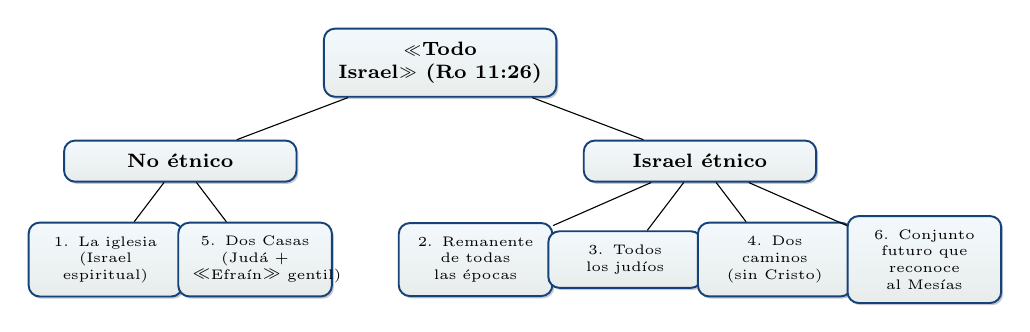
\begin{tikzpicture}[level distance=1.25cm,
  level 1/.style={sibling distance=6.6cm},
  level 2/.style={sibling distance=1.9cm},
  every node/.style={caja,align=center,text width=1.6cm,font=\tiny}]
\node[text width=2.6cm,font=\scriptsize\bfseries,fill=oro!25] {«Todo Israel» (Ro 11:26)}
  child {node[text width=2.6cm,font=\scriptsize\bfseries] {No étnico}
    child {node {1. La iglesia (Israel espiritual)}}
    child {node {5. Dos Casas (Judá + «Efraín» gentil)}}}
  child {node[text width=2.6cm,font=\scriptsize\bfseries] {Israel étnico}
    child {node {2. Remanente de todas las épocas}}
    child {node {3. Todos los judíos}}
    child {node {4. Dos caminos (sin Cristo)}}
    child {node[fill=oro!25] {6. Conjunto futuro que reconoce al Mesías}}};
\end{tikzpicture}\par
\elabpropia\vspace{4pt}
{\small Tres grandes posturas con sus variantes, más la de los «dos caminos».}
\end{frame}

\begin{frame}{1. La iglesia como Israel}
\begin{columns}[T,onlytextwidth]
\begin{column}{0.49\textwidth}\small\RaggedRight
\textbf{\textcolor{cafe}{Exposición}}\par
«Extiendo el nombre de Israel a todo el pueblo de Dios» (Calvino, 1540/1849). Wright (2013): Israel redefinido en torno al Mesías. En esta familia: las promesas se cumplen en la iglesia. Reemplazo estricto: Justino (\emph{Diálogo} 11, 135).\par\smallskip
\textbf{\textcolor{cafe}{Fortaleza}}: unidad en Cristo (Ef 2:14--16; Gá 3:28--29).
\end{column}
\begin{column}{0.49\textwidth}\scriptsize\RaggedRight
\textbf{\textcolor{ladrillo}{Debilidades}}
\begin{itemize}
\item En 11:25 «Israel» se distingue de «las naciones»; un cambio de sentido en 11:26 resulta improbable.
\item El «cuánto más» (11:12, 15) pierde sentido.
\item La irrevocabilidad se dice del Israel \emph{no creyente} (11:28--29).
\item Desarraiga Jer 31:35--37; Ez 36:24--28; Am 9:14--15.
\item El olivo enseña injerto, no reemplazo (11:17, 24).
\end{itemize}
\end{column}
\end{columns}
\end{frame}

\begin{frame}{2--4. Remanente, todos, dos caminos}
\begin{columns}[T,onlytextwidth]
\begin{column}{0.32\textwidth}\scriptsize\RaggedRight
\textbf{\textcolor{ladrillo}{2. Remanente de todas las épocas}}\par\smallskip
Hendriksen (1981); Robertson (2000); Núñez (s.\,f.).\par\smallskip
\textbf{A favor}: «Israel» étnico; doctrina del remanente.\par
\textbf{En contra}: 11:26 repetiría 11:5; no habría «misterio»; ignora «hasta que» y la «plenitud» frente al remanente.
\end{column}
\begin{column}{0.32\textwidth}\scriptsize\RaggedRight
\textbf{\textcolor{ladrillo}{3. Todos los judíos}}\par\smallskip
Sin respaldo exegético serio.\par\smallskip
\textbf{En contra}: Ro 9:6--8; 10:1 (Pablo ora por su salvación); 11:23 («si no permanecen en incredulidad»). La Mishná misma pone excepciones.
\end{column}
\begin{column}{0.33\textwidth}\scriptsize\RaggedRight
\textbf{\textcolor{ladrillo}{4. Dos caminos (\emph{Sonderweg})}}\par\smallskip
Stendahl (1976); Gaston (1987); Gager (2000): Israel salvado por su pacto, sin fe en Jesús.\par\smallskip
\textbf{A favor}: rechaza el desprecio cristiano a Israel.\par
\textbf{En contra}: Ro 10:9--13 («no hay diferencia»); 11:23; el Libertador es Jesús (1~Ts 1:10); Fil 3:4--9.
\end{column}
\end{columns}
\end{frame}

\begin{frame}{5. Las Dos Casas}
\begin{columns}[T,onlytextwidth]
\begin{column}{0.47\textwidth}\centering
{\scriptsize\textbf{\textcolor{cafe}{La propuesta}} (Koniuchowsky, 2003)}\par\smallskip
\begin{tikzpicture}[node distance=0.25cm and 0.3cm]
\node[bloque,text width=2.0cm] (n) {Israel, reino del norte (Efraín, Samaria)};
\node[bloque,text width=2.0cm,right=of n] (s) {Judá, reino del sur (Jerusalén)};
\node[bloqueoro,text width=2.0cm,below=of n] (d) {Dispersión asiria (722 a.\,e.\,c.) $\to$ «entre las naciones»};
\node[bloqueoro,text width=2.0cm,below=of s] (p) {«Plenitud de los gentiles» = \heb{מְלֹא־הַגּוֹיִם} (Gn 48:19)};
\node[bloqueazul,text width=4.6cm,below=0.35cm of $(d.south)!0.5!(p.south)$] (t) {«Todo Israel» = Judá + Efraín (Ez 37:15--28)};
\draw[flecha] (n)--(d); \draw[flecha] (d)--(p);
\draw[flecha] (d.south) -- (d.south |- t.north);
\draw[flecha] (p.south) -- (p.south |- t.north);
\end{tikzpicture}\elabpropia
\begin{clave}\textbf{Fortalezas}: rechaza el reemplazo; toma en serio Ez 37 y Zac 12:10.\end{clave}
\end{column}
\begin{column}{0.51\textwidth}\scriptsize\RaggedRight
\textbf{\textcolor{ladrillo}{Debilidades}}
\begin{enumerate}
\item Los gentiles son \grc{κατὰ φύσιν ἀγριέλαιος}, silvestres \emph{por naturaleza} (11:24).
\item Inclusión por fe, no por linaje (Ro 9:24; Ef 2:11--13).
\item Os 2:23 en Ro 9:25--26: analogía, no genealogía.
\item LXX de Gn 48:19: \grc{πλῆθος}, no \grc{πλήρωμα}.
\item Muchos del norte se integraron en Judá (2~Cr 11:13--17; 15:9; 30:1--11); Ana, de Aser (Lc 2:36); «nuestras doce tribus» (Hch 26:7).
\item Sin evidencia que identifique pueblos gentiles con las tribus.
\end{enumerate}
\end{column}
\end{columns}
\end{frame}

\begin{frame}{6. Israel étnico futuro}
\begin{columns}[T,onlytextwidth]
\begin{column}{0.49\textwidth}\small\RaggedRight
\textbf{\textcolor{cafe}{Exposición}}\par
El pueblo judío como conjunto, no cada individuo, reconocerá a Jesús como Mesías cuando entre la plenitud de las naciones: Murray (1965); Cranfield (1979); Dunn (1988); Morris (1988); Fitzmyer (1993); Stott (1994); Moo (1996); Schreiner (1998); ya Moule (1894).\par\smallskip
{\scriptsize Murray: es \textbf{exegéticamente imposible} dar a «Israel» en 11:26 otro sentido que el del capítulo; Stott lo suscribe.}\par\smallskip
\textbf{\textcolor{cafe}{Debilidad}}: descansa en un cumplimiento futuro que Pablo no detalla; exige articular lo colectivo con lo individual (el conjunto lo forman individuos que creen).
\end{column}
\begin{column}{0.49\textwidth}\scriptsize\RaggedRight
\textbf{\textcolor{ladrillo}{Fortalezas}}
\begin{itemize}
\item Mismo sentido de «Israel» en 11:25 y 11:26.
\item Explica «hasta que», remanente/plenitud y «cuánto más».
\item Reinjerto condicionado a la fe (11:23).
\item Uso colectivo de \emph{kol Yisra'el}.
\item Is 59 y Jer 31: pacto con Jacob/Israel.
\item Jesús: «no me veréis más hasta que digáis: Bendito el que viene» (Mt 23:39); Lc 21:24.
\end{itemize}
\end{column}
\end{columns}
\end{frame}

\begin{frame}{Tabla comparativa}
\centering\scriptsize\renewcommand{\arraystretch}{1.3}
\begin{tabular}{>{\RaggedRight\arraybackslash}p{3.8cm}>{\centering\arraybackslash}p{0.95cm}>{\centering\arraybackslash}p{0.95cm}>{\centering\arraybackslash}p{0.95cm}>{\centering\arraybackslash}p{0.95cm}>{\centering\arraybackslash}p{0.95cm}>{\centering\arraybackslash}p{0.95cm}}
\toprule
\color{ladrillo}\bfseries Criterio (Ro 11) & \textbf{1. Iglesia} & \textbf{2. Rema\-nente} & \textbf{3. Todos} & \textbf{4. Dos caminos} & \textbf{5. Dos Casas} & \textbf{6. Israel futuro}\\\midrule
Mismo «Israel» en 11:25 y 26 & no & sí & sí & sí & no & \textbf{sí}\\
Explica «hasta que» & no & no & parcial & sí & sí & \textbf{sí}\\
Plenitud mayor que remanente (11:12, 15) & no & no & sí & sí & parcial & \textbf{sí}\\
Exige fe (10:9--13; 11:23) & sí & sí & no & no & sí & \textbf{sí}\\
Gentiles, olivo silvestre (11:24) & parcial & sí & sí & sí & no & \textbf{sí}\\
Irrevocable para el Israel no creyente (11:28--29) & no & parcial & sí & sí & parcial & \textbf{sí}\\
\bottomrule
\end{tabular}\par
\elabpropia\vspace{6pt}
\begin{clave}Solo la postura 6 cumple los seis criterios del capítulo; la 4 falla en el que Pablo repite con más fuerza: la fe (10:9--13; 11:23).\end{clave}
\end{frame}

\begin{frame}{Tres familias: fortalezas y debilidades}
\centering\small\renewcommand{\arraystretch}{1.35}
\begin{tabular}{>{\RaggedRight\arraybackslash}p{2.8cm}>{\RaggedRight\arraybackslash}p{4.0cm}>{\RaggedRight\arraybackslash}p{4.4cm}}
\toprule
\color{ladrillo}\bfseries Postura & \color{ladrillo}\bfseries Fortaleza & \color{ladrillo}\bfseries Debilidad\\\midrule
Israel espiritual & Unidad en Cristo & Ignora la dimensión literal y nacional\\
Dos Casas & Cumplimiento literal; Judá e Israel & Gentiles como Efraín: especulativo\\
Israel étnico con Mesías & Literal y espiritual; integra a los gentiles & Depende de un cumplimiento futuro\\
\bottomrule
\end{tabular}\par
\elabpropia\vspace{6pt}
\begin{notalam}[Precisión: «Israel» en las Dos Casas]
En esta postura «Israel» se usa en dos sentidos que conviene no confundir: el \textbf{pueblo completo} (Ro 9--11) y el \textbf{reino del norte} (Efraín, capital Samaria), dispersado por Asiria. Pablo usa siempre el primero; muchos del norte ya se habían integrado en Judá (2~Cr 11:13--17; 30:1--11), y Ana era de Aser (Lc 2:36).
\end{notalam}
\end{frame}

\begin{frame}{Conclusión sobre «todo Israel»}
\begin{tcolorbox}[colback=piedra,colframe=ladrillo,boxrule=1pt,arc=3pt,fontupper=\small]
La lectura más consistente con el contexto de Romanos 11 es la \textbf{restauración futura del Israel étnico como conjunto, que reconocerá al Mesías}.
\end{tcolorbox}
\begin{columns}[T,onlytextwidth]
\begin{column}{0.44\textwidth}\small
\begin{itemize}
\item \textbf{No cada individuo}: colectivo, como en el AT y la Mishná.
\item \textbf{No por etnia sin fe}: «si no permanecen en incredulidad» (11:23).
\item \textbf{No en reemplazo de la iglesia}: un solo olivo.
\end{itemize}
\end{column}
\begin{column}{0.53\textwidth}
\begin{cita}[fontupper=\scriptsize\itshape]«Todo Israel» significa un futuro volverse masivo del pueblo judío a Yeshúa como Mesías, no la salvación de cada judío individual. Israel es ampliado, no reemplazado.\fuente{(ONE FOR ISRAEL, 2025; síntesis)}\end{cita}
\scriptsize Según estima el ministerio, c. 1 millón de judíos creyentes entre c. 15 millones: hoy, como entonces, un remanente.
\end{column}
\end{columns}
\end{frame}

\begin{frame}{Lo que queda abierto}
\begin{columns}[T,onlytextwidth]
\begin{column}{0.32\textwidth}\small\RaggedRight
\textbf{\textcolor{ladrillo}{El momento}}\par\smallskip
Pablo no fecha la plenitud ni la salvación de Israel. «No os toca saber los tiempos» (Hch 1:7).
\end{column}
\begin{column}{0.33\textwidth}\small\RaggedRight
\textbf{\textcolor{ladrillo}{La parusía}}\par\smallskip
¿El Libertador de Sion es la segunda venida? Zac 12:10 («mirarán a mí, a quien traspasaron»); Mt 23:39; Hch 3:19--21 (\grc{ἀποκατάστασις πάντων}).
\end{column}
\begin{column}{0.32\textwidth}\small\RaggedRight
\textbf{\textcolor{ladrillo}{La tierra}}\par\smallskip
Ro 11 no la menciona; los profetas sí (Ez 36--37; Jer 31:38--40). Leer 1948 como Ez 37:1--8 es una interpretación teológica, no una afirmación de Romanos.
\end{column}
\end{columns}\vspace{8pt}
\centering
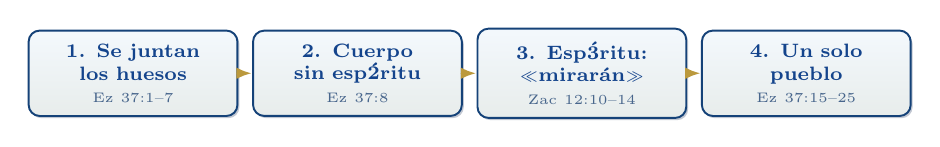
\begin{tikzpicture}[node distance=0.25cm]
\foreach \i/\t/\r in {1/{Se juntan los huesos}/{Ez 37:1--7},2/{Cuerpo sin espíritu}/{Ez 37:8},3/{Espíritu: «mirarán»}/{Zac 12:10--14},4/{Un solo pueblo}/{Ez 37:15--25}}{
  \node[caja,text width=2.3cm,align=center] (e\i) at (\i*2.85,0) {\textbf{\textcolor{ladrillo}{\i. \t}}\\{\tiny\color{sepia}\r}};}
\foreach \a/\b in {1/2,2/3,3/4}{\draw[-{Latex[length=2mm]},oro!90!ladrillo,line width=1.2pt] (e\a) -- (e\b);}
\end{tikzpicture}\par
\elabpropia
\end{frame}

% ===================================================
\section{Hilos}
\begin{frame}{Siete estudios, un capítulo}
\centering\scriptsize\renewcommand{\arraystretch}{1.12}
\begin{tabular}{>{\RaggedRight\arraybackslash}p{2.0cm}>{\RaggedRight\arraybackslash}p{3.4cm}>{\RaggedRight\arraybackslash}p{2.4cm}>{\RaggedRight\arraybackslash}p{3.4cm}}
\toprule
\color{ladrillo}\bfseries Estudio & \color{ladrillo}\bfseries Hilo & \color{ladrillo}\bfseries Textos & \color{ladrillo}\bfseries En Romanos 11\\\midrule
1. Abraham--Éxodo & Pacto perpetuo; remanente de José & Gn 15; 17:7; 45:7 & Raíz santa (11:16); amados por los padres (11:28)\\
2. Éxodo--Josué & Reino de sacerdotes; celos & Éx 19:6; Dt 29:4; 32:21 & Celos (11:11, 14); ojos que no ven (11:8)\\
3. Jueces--David & YHWH no desampara; Benjamín & 1~S 12:22 & «¿Ha desechado Dios?» (11:1)\\
4. David--división & Pacto davídico; raíz de Isaí & 2~S 7; Is 11:10 & David testigo (11:9); Ro 15:12\\
5. Reyes y cautiverios & Elías en el norte; «no pueblo mío»; nuevo pacto; Ez 37 & 1~R 19:18; Os 1--2; Jer 31 & Siete mil (11:4); pacto (11:27); irrevocable (11:29)\\
6. Segundo Templo & Redentor de Sion; «todo Israel» confiesa & Is 59:20; Dn 9:11 & «Vendrá de Sion» (11:26)\\
7. Cristo--año 70 & Remanente; «hasta que» & Hch 21:20; Lc 21:24; Mt 23:39 & Remanente (11:5); «hasta que» (11:25)\\
\bottomrule
\end{tabular}\par
\elabpropia
\end{frame}

\begin{frame}{Tres hilos mayores}
\begin{columns}[c,onlytextwidth]
\begin{column}{0.50\textwidth}
\centering
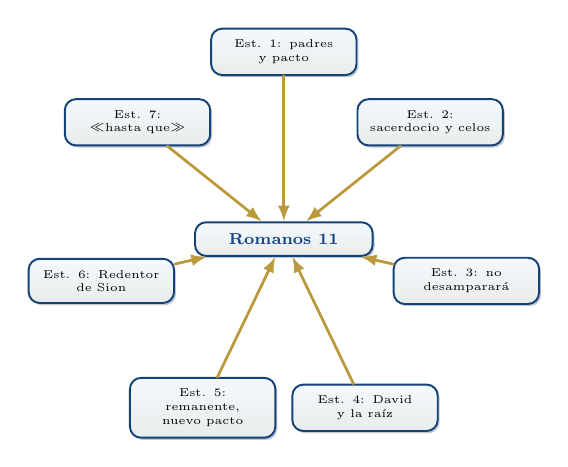
\begin{tikzpicture}[scale=0.82,transform shape]
\node[caja,fill=oro!25,text width=2.4cm,align=center,font=\scriptsize\bfseries] (r) at (0,0) {\textcolor{ladrillo}{Romanos 11}};
\foreach \ang/\n/\t in {90/1/{1: padres y pacto},38.6/2/{2: sacerdocio y celos},-12.9/3/{3: no desamparará},-64.3/4/{4: David y la raíz},-115.7/5/{5: remanente, nuevo pacto},-167.1/6/{6: Redentor de Sion},141.4/7/{7: «hasta que»}}{
  \node[caja,text width=1.9cm,align=center,font=\tiny] (n\n) at (\ang:2.9) {Est. \t};
  \draw[-{Latex[length=2mm]},oro!90!ladrillo,line width=1pt] (n\n) -- (r);}
\end{tikzpicture}\elabpropia
\end{column}
\begin{column}{0.47\textwidth}\small
\begin{enumerate}
\item \destacar{Remanente}: José (Gn 45:7), Elías (1~R 19:18), «un resto volverá» (Is 10:21), el retorno (Esd 9:8), Hch 21:20, Pablo.
\item \destacar{Reunificación}: Judá y José, «un solo palo» (Ez 37:15--28). Para Pablo, «Israel» ya hereda a todas las tribus.
\item \destacar{Nuevo pacto}: Jer 31; Ez 36 $\to$ Lc 22:20 $\to$ Ro 11:27.
\end{enumerate}
\end{column}
\end{columns}
\end{frame}

% ===================================================
\section{Tradición judía}
\begin{frame}{La Mishná: «todo Israel»}
\begin{columns}[T,onlytextwidth]
\begin{column}{0.52\textwidth}
\centering{\heb{כל ישראל יש להם חלק לעולם הבא}}\par\smallskip
\begin{cita}[fontupper=\scriptsize\itshape]Todo Israel tiene parte en el mundo venidero, porque está dicho: «Tu pueblo, todos ellos justos» (Is 60:21). Y estos no tienen parte: el que niega la resurrección [\ldots], el que dice que la Torá no es del cielo, y el epicúreo.\fuente{(Mishná, Sanedrín 10:1)}\end{cita}
\scriptsize 10:2 añade Jeroboam, Acab, Manasés, Balaam, Doeg, Ajitófel y Guejazí. \destacar{«Todo Israel»: un colectivo que admite excepciones.}
\end{column}
\begin{column}{0.45\textwidth}\small\RaggedRight
\textbf{\textcolor{cafe}{Las diez tribus (Sanedrín 10:3)}}\par\smallskip
R. Aquiba: «las diez tribus no volverán» (Dt 29:28 [29:27]).\par\smallskip
R. Eliézer: como el día que se oscurece y vuelve a aclarar, así vendrá la luz para ellas.\par\medskip
\begin{notalam}[Precisión: fecha y texto]
Mishná c. 200 e.\,c.: posterior a Pablo. Algunos manuscritos no traen la frase inicial; verificar en edición crítica. Is 60:21 sigue a Is 59:20--21.
\end{notalam}
\end{column}
\end{columns}
\end{frame}

\begin{frame}{Talmud, Targum y liturgia}
\begin{columns}[T,onlytextwidth]
\begin{column}{0.49\textwidth}\scriptsize\RaggedRight
\textbf{\textcolor{ladrillo}{Sanedrín 97b--98a}} (tradiciones posteriores)
\begin{itemize}
\item R. Eliézer: «si Israel se arrepiente, es redimido».
\item Is 60:22: «si lo merecen, lo apresuraré; si no, a su tiempo» (R. Josué ben Leví).
\item El Mesías responde «hoy»: Sal 95:7, «si oís su voz».
\item R. Yojanán: angustias como un río $\to$ «vendrá a Sion el Redentor» (Is 59:19--20).
\end{itemize}
\textbf{\textcolor{ladrillo}{Targum de Is 59:20}}: el redentor viene para hacer volver a la Torá a los rebeldes de Jacob (Chilton, 1987).
\end{column}
\begin{column}{0.49\textwidth}\scriptsize\RaggedRight
\textbf{\textcolor{ladrillo}{\emph{U-va le-Tsiyyón}}}: Is 59:20--21 abre una oración del servicio diario de la mañana.\par\smallskip
\textbf{\textcolor{ladrillo}{La Amidá}}\par\smallskip
\renewcommand{\arraystretch}{1.2}
\begin{tabular}{>{\RaggedRight\arraybackslash}p{1.3cm}>{\RaggedRight\arraybackslash}p{3.6cm}}
\toprule
10.ª & «Reúnes a los dispersos de tu pueblo Israel» (Is 11:12; Ez 37:21)\\
14.ª & «Edificas Jerusalén» (Lc 21:24)\\
15.ª & «Haz brotar el renuevo de David» (Jer 23:5; Ro 15:12)\\
\bottomrule
\end{tabular}\par
\notafig{Elaboración propia a partir de Sacks (2009).}
\end{column}
\end{columns}
\end{frame}

\begin{frame}{Israel como olivo}
\begin{columns}[c,onlytextwidth]
\begin{column}{0.52\textwidth}
\centering{\large\heb{זַיִת רַעֲנָן יְפֵה פְרִי־תֹאַר}}\par\smallskip
\begin{cita}Olivo verde, hermoso en fruto y en aspecto, llamó YHWH tu nombre; [\ldots] y quebraron sus ramas.\fuente{(Jer 11:16)}\end{cita}
\end{column}
\begin{column}{0.45\textwidth}
\begin{cita}[fontupper=\scriptsize\itshape]¿Por qué Israel es comparado con el olivo? Así como las hojas del olivo no caen ni en verano ni en invierno, así Israel no será desechado nunca, ni en este mundo ni en el venidero.\fuente{(Talmud, Menajot 53b, R. Josué ben Leví)}\end{cita}
\end{column}
\end{columns}\vspace{4pt}
\centering
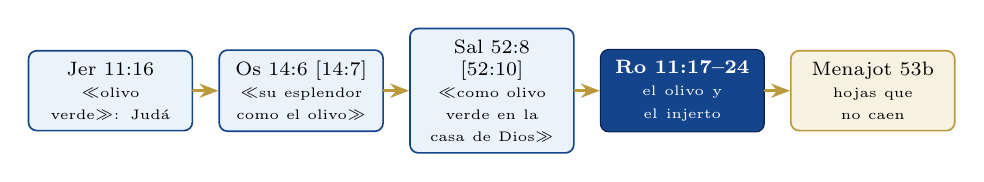
\begin{tikzpicture}[node distance=0.32cm]
\node[bloque,text width=1.8cm] (a) {Jer 11:16\\{\tiny «olivo verde»: Judá}};
\node[bloque,text width=1.8cm,right=of a] (b) {Os 14:6 [14:7]\\{\tiny «su esplendor como el olivo»}};
\node[bloque,text width=1.8cm,right=of b] (c) {Sal 52:8 [52:10]\\{\tiny «como olivo verde en la casa de Dios»}};
\node[bloqueazul,text width=1.8cm,right=of c] (d) {Ro 11:17--24\\{\tiny\mdseries el olivo y el injerto}};
\node[bloqueoro,text width=1.8cm,right=of d] (e) {Menajot 53b\\{\tiny hojas que no caen}};
\foreach \u/\v in {a/b,b/c,c/d,d/e}{\draw[flecha] (\u)--(\v);}
\end{tikzpicture}\elabpropia
{\small\itshape\color{sepia}\centering Un olivo que pierde ramas, pero que nadie arranca: Pablo habla aquí el idioma de Israel.\par}
\end{frame}

% ===================================================
\section{Implicaciones}
\begin{frame}{Para la iglesia de las naciones}
\centering
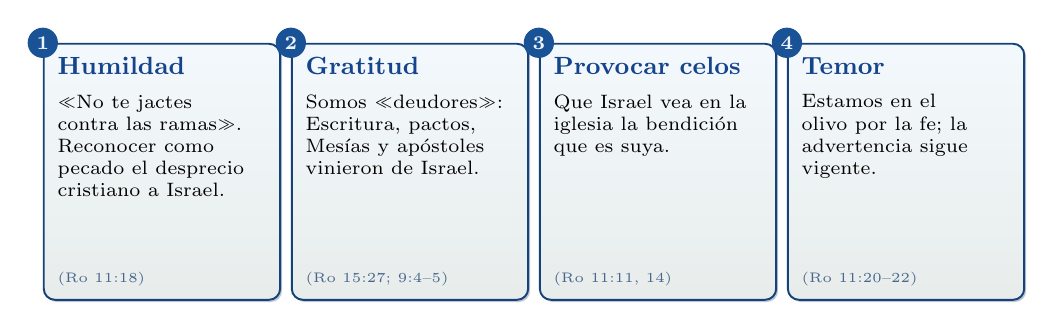
\begin{tikzpicture}
 \foreach \x/\n/\t/\d/\r in {0/1/{Humildad}/{«No te jactes contra las ramas». Reconocer como pecado el desprecio cristiano a Israel.}/{Ro 11:18},
   3.15/2/{Gratitud}/{Somos «deudores»: Escritura, pactos, Mesías y apóstoles vinieron de Israel.}/{Ro 15:27; 9:4--5},
   6.3/3/{Provocar celos}/{Que Israel vea en la iglesia la bendición que es suya.}/{Ro 11:11, 14},
   9.45/4/{Temor}/{Estamos en el olivo por la fe; la advertencia sigue vigente.}/{Ro 11:20--22}}{
  \node[caja,anchor=north] (b\n) at (\x,0) {\parbox[t][2.9cm][t]{2.65cm}{\RaggedRight
    {\small\textbf{\textcolor{ladrillo}{\t}}}\\[4pt]\scriptsize \d\par\vfill{\tiny\color{sepia}(\r)}}};
  \node[circle,fill=cafe,text=piedra,font=\scriptsize\bfseries,inner sep=1.6pt] at (b\n.north west) {\n};}
\end{tikzpicture}\par
\elabpropia\vspace{6pt}
\begin{clave}«No sustentas tú a la raíz, sino la raíz a ti» (11:18): la fe de las naciones depende de la historia de Israel, no al revés.\end{clave}
\end{frame}

\begin{frame}{Contra el desprecio a Israel}
\begin{columns}[c,onlytextwidth]
\begin{column}{0.55\textwidth}
\begin{cita}[fontupper=\small\itshape]Qué extraño que Dios eligiera a los judíos.\fuente{(atribuido a W. N. Ewer)}\end{cita}
\begin{cita}[fontupper=\small\itshape]Pero no tan extraño como los que eligen al Dios judío y desprecian a los judíos.\fuente{(atribuido a C. Browne)}\end{cita}
\end{column}
\begin{column}{0.42\textwidth}\scriptsize\RaggedRight
\begin{itemize}
\item «No te jactes contra las ramas» (Ro 11:18).
\item «De los cuales, según la carne, vino Cristo» (Ro 9:5): el Libertador viene de Sion.
\item «La salvación viene de los judíos» (Jn 4:22).
\item Jonás se enojó porque Dios perdonó a Nínive (Jon 4:1--2); molestarse por la misericordia a Israel es su error invertido.
\end{itemize}
\end{column}
\end{columns}
\end{frame}

\begin{frame}{Israel hoy y la esperanza}
\begin{columns}[T,onlytextwidth]
\begin{column}{0.49\textwidth}\small\RaggedRight
\textbf{\textcolor{cafe}{Teología, no política}}\par\smallskip
Ro 11 trata del pueblo de Israel ante Dios y el Mesías, no de un programa político. Amar a Israel «por causa de los padres» no supone aprobar cada acción de un gobierno; también los profetas amaban a Israel y denunciaban a sus reyes. La indiferencia, sin embargo, queda excluida (Jer 31:35--37).
\end{column}
\begin{column}{0.49\textwidth}
\textbf{\small\textcolor{cafe}{La esperanza}}\par\smallskip
\begin{cita}[fontupper=\scriptsize\itshape]El anhelo de mi corazón y mi oración a Dios por Israel es para salvación.\fuente{(Ro 10:1)}\end{cita}
\small Hacia donde se encamina la historia: la plenitud de las naciones y la de Israel.
\end{column}
\end{columns}
\end{frame}

% ===================================================
\section{Síntesis}
\begin{frame}{Síntesis}
\begin{tcolorbox}[colback=piedra,colframe=ladrillo,boxrule=1pt,arc=3pt,fontupper=\small]
\textbf{\textcolor{cafe}{Romanos 11:}} Dios no ha desechado a su pueblo. Existe hoy un remanente escogido por gracia, mientras el resto permanece endurecido en parte y por un tiempo, de modo que entren las naciones y Israel sea provocado a celos. Cuando haya entrado la plenitud de las naciones, todo Israel será salvo por el Libertador de Sion y el nuevo pacto, porque los dones y el llamamiento de Dios son irrevocables.
\end{tcolorbox}
\scriptsize\renewcommand{\arraystretch}{1.2}
\begin{tabular}{>{\RaggedRight\arraybackslash}p{2.4cm}>{\RaggedRight\arraybackslash}p{8.9cm}}
\toprule
\color{ladrillo}\bfseries Dimensión & \color{ladrillo}\bfseries Aporte\\\midrule
Histórica & Roma tras el edicto de Claudio: Pablo corrige la arrogancia gentil (11:13--25)\\
Literaria & Ro 9--11 es una unidad; cuatro pasos: remanente, tropiezo, misterio, doxología\\
Filológica & \grc{πώρωσις ἀπὸ μέρους}, \grc{ἄχρι οὗ}, \grc{πλήρωμα}, \grc{καὶ οὕτως}, \grc{πᾶς Ἰσραήλ}, \grc{ἐκ Σιών}\\
Teológica & Fidelidad de Dios; inclusión sin reemplazo; salvación futura del Israel étnico por la fe\\
\bottomrule
\end{tabular}\par
\elabpropia
\end{frame}

\begin{frame}{La doxología de la serie}
\fotolado{panel_ro33.jpg}{Elaboración propia: Ro 11:33--34a en escritura uncial (texto NA28).}
\begin{columns}[c,onlytextwidth]
\begin{column}{0.57\textwidth}
\small La serie partió de Gn 15:5, «mira los cielos y cuenta las estrellas», y concluye con un apóstol de la tribu de Benjamín ante el plan de Dios:
\begin{cita}¡Oh profundidad de las riquezas, y de la sabiduría y del conocimiento de Dios! ¡Cuán insondables son sus juicios e inescrutables sus caminos! [\ldots] Porque de él, por él y para él son todas las cosas. A él sea la gloria por los siglos. Amén.\fuente{(Ro 11:33, 36)}\end{cita}
\end{column}
\begin{column}{0.41\textwidth}\end{column}
\end{columns}
\end{frame}

\begin{frame}{Para la reflexión}
\small
\begin{enumerate}
\item Pablo prueba la fidelidad de Dios con su propia persona (11:1). ¿Qué significa que la prueba sea alguien del remanente?
\item El endurecimiento es parcial, temporal y con propósito. ¿Cómo cambia esto la manera de hablar del pueblo judío?
\item ¿Qué formas de «jactancia contra las ramas» reconoce en la historia de la iglesia y en su comunidad (11:18--22)?
\item ¿Qué versículos de Ro 11 son decisivos para elegir entre «la iglesia» y «el Israel étnico futuro»?
\item La Mishná dice «todo Israel» y enumera excepciones. ¿Qué enseña sobre la frase de Pablo?
\item ¿Qué significa, en la práctica, ser «deudores» de Israel (Ro 15:27)?
\end{enumerate}
\end{frame}

% ===================================================
\section{Glosario y fuentes}
\begin{frame}{Glosario}
\begin{columns}[T,onlytextwidth]
\begin{column}{0.49\textwidth}\scriptsize
\textbf{Agriélaios} (\grc{ἀγριέλαιος}): olivo silvestre (11:17, 24).\par\smallskip
\textbf{Ametamélēta} (\grc{ἀμεταμέλητα}): irrevocables (11:29).\par\smallskip
\textbf{Aparchḗ} (\grc{ἀπαρχή}): primicia; \heb{רֵאשִׁית} (11:16).\par\smallskip
\textbf{Enkentrízō} (\grc{ἐγκεντρίζω}): injertar (11:17--24).\par\smallskip
\textbf{Go'el} (\heb{גֹּאֵל}): redentor (Is 59:20).\par\smallskip
\textbf{Jéleq} (\heb{חֵלֶק}): parte en el mundo venidero (Mishná).\par\smallskip
\textbf{Kaì hoútōs} (\grc{καὶ οὕτως}): «y así» (11:26).\par\smallskip
\textbf{Kol Yisra'el} (\heb{כָּל־יִשְׂרָאֵל}): todo Israel, colectivo.\par\smallskip
\textbf{Leîmma} (\grc{λεῖμμα}): remanente (11:5).\par\smallskip
\textbf{Mḕ génoito} (\grc{μὴ γένοιτο}): «¡de ningún modo!».
\end{column}
\begin{column}{0.49\textwidth}\scriptsize
\textbf{Mystḗrion} (\grc{μυστήριον}): designio revelado (11:25).\par\smallskip
\textbf{Parazēlóō} (\grc{παραζηλόω}): provocar a celos (11:11).\par\smallskip
\textbf{Pâs Israḗl} (\grc{πᾶς Ἰσραήλ}): todo Israel (11:26).\par\smallskip
\textbf{Plḗrōma} (\grc{πλήρωμα}): plenitud (11:12, 25).\par\smallskip
\textbf{Pṓrōsis} (\grc{πώρωσις}): endurecimiento (11:25).\par\smallskip
\textbf{Próslēmpsis} (\grc{πρόσλημψις}): aceptación (11:15).\par\smallskip
\textbf{She'erit} (\heb{שְׁאֵרִית}): remanente (Gn 45:7).\par\smallskip
\textbf{Sōthḗsetai} (\grc{σωθήσεται}): será salvo (11:26).\par\smallskip
\textbf{U-va le-Tsiyyón} (\heb{ובא לציון}): «y vendrá a Sion».\par\smallskip
\textbf{Zayit} (\heb{זַיִת}): olivo; Israel (Jer 11:16).
\end{column}
\end{columns}
\end{frame}

\begin{frame}[allowframebreaks]{Referencias}
\tiny
\refapa{Baxter, A.~G., \& Ziesler, J.~A. (1985). Paul and arboriculture: Romans 11.17--24. \emph{Journal for the Study of the New Testament, 8}(24), 25--32.}
\refapa{Beale, G.~K., \& Carson, D.~A. (Eds.). (2007). \emph{Commentary on the New Testament use of the Old Testament}. Baker Academic.}
\refapa{\emph{Biblia Hebraica Stuttgartensia} (5.ª ed.). (1997). Deutsche Bibelgesellschaft.}
\refapa{Biblical Studies Press. (2019). \emph{NET Bible} (2.ª ed.), nota textual a Romanos 11:31. \url{https://netbible.org}}
\refapa{Bruno, C.~R. (2008). The Deliverer from Zion: The source(s) and function of Paul's citation in Romans 11:26--27. \emph{Tyndale Bulletin, 59}(1), 119--134.}
\refapa{Calvino, J. (1849). \emph{Commentaries on the epistle of Paul the apostle to the Romans} (J. Owen, Trad.). Calvin Translation Society. (Obra original publicada en 1540)}
\refapa{Chilton, B.~D. (1987). \emph{The Isaiah Targum} (The Aramaic Bible, Vol. 11). Michael Glazier.}
\refapa{Cranfield, C.~E.~B. (1979). \emph{A critical and exegetical commentary on the epistle to the Romans} (Vol. 2). T\&T Clark.}
\refapa{Danby, H. (Trad.). (1933). \emph{The Mishnah}. Oxford University Press.}
\refapa{Das, A.~A. (2007). \emph{Solving the Romans debate}. Fortress Press.}
\refapa{Dunn, J.~D.~G. (1988). \emph{Romans 9--16} (Word Biblical Commentary, Vol. 38B). Word Books.}
\refapa{Epstein, I. (Ed.). (1935--1948). \emph{The Babylonian Talmud}. Soncino Press.}
\refapa{Fitzmyer, J.~A. (1993). \emph{Romans} (The Anchor Bible, Vol. 33). Doubleday.}
\refapa{Gager, J.~G. (2000). \emph{Reinventing Paul}. Oxford University Press.}
\refapa{Gaston, L. (1987). \emph{Paul and the Torah}. University of British Columbia Press.}
\refapa{Hays, R.~B. (1989). \emph{Echoes of Scripture in the letters of Paul}. Yale University Press.}
\refapa{Hendriksen, W. (1981). \emph{Exposition of Paul's epistle to the Romans}. Baker.}
\refapa{Jewett, R. (2007). \emph{Romans: A commentary} (Hermeneia). Fortress Press.}
\refapa{Kaiser, W.~C. (1998). \emph{The Messiah in the Old Testament}. Zondervan.}
\refapa{Koniuchowsky, M.~Y. (2003). \emph{The Restoration Scriptures: True Name Edition}. Your Arms to Israel.}
\refapa{Moo, D.~J. (1996). \emph{The epistle to the Romans}. Eerdmans.}
\refapa{Morris, L. (1988). \emph{The epistle to the Romans}. Eerdmans.}
\refapa{Moule, H.~C.~G. (1894). \emph{The epistle of St. Paul to the Romans}. Hodder \& Stoughton.}
\refapa{Murray, J. (1965). \emph{The epistle to the Romans} (Vol. 2). Eerdmans.}
\refapa{Nanos, M.~D. (1996). \emph{The mystery of Romans: The Jewish context of Paul's letter}. Fortress Press.}
\refapa{Núñez, M. (s.\,f.). [Exposición de Romanos 11] [Video]. YouTube.}
\refapa{\emph{Novum Testamentum Graece} (28.ª ed.). (2012). Deutsche Bibelgesellschaft.}
\refapa{ONE FOR ISRAEL Ministry. (2025, 3 de julio). \emph{What does «all Israel will be saved» mean in Romans 11?} \url{https://www.oneforisrael.org/what-does-all-israel-will-be-saved-mean-in-romans-11/}}
\refapa{Predicación sobre Romanos 11:25--32: «El misterio revelado». (s.\,f.). [Transcripción].}
\refapa{Rahlfs, A., \& Hanhart, R. (Eds.). (2006). \emph{Septuaginta} (ed. rev.). Deutsche Bibelgesellschaft.}
\refapa{Robertson, O.~P. (2000). \emph{The Israel of God: Yesterday, today, and tomorrow}. P\&R Publishing.}
\refapa{Sacks, J. (Trad.). (2009). \emph{The Koren Siddur}. Koren Publishers.}
\refapa{Sanders, E.~P. (1977). \emph{Paul and Palestinian Judaism}. Fortress Press.}
\refapa{Schreiner, T.~R. (1998). \emph{Romans} (Baker Exegetical Commentary on the New Testament). Baker Academic.}
\refapa{Stanley, C.~D. (1992). \emph{Paul and the language of Scripture}. Cambridge University Press.}
\refapa{Stendahl, K. (1976). \emph{Paul among Jews and Gentiles}. Fortress Press.}
\refapa{Stott, J.~R.~W. (1994). \emph{The message of Romans}. InterVarsity Press.}
\refapa{Stowers, S.~K. (1981). \emph{The diatribe and Paul's letter to the Romans}. Scholars Press.}
\refapa{Suetonio. (1914). \emph{The lives of the Caesars} (J.~C. Rolfe, Trad.). Harvard University Press.}
\refapa{van der Horst, P.~W. (2000). «Only then will all Israel be saved»: A short note on the meaning of \emph{kai houtōs} in Romans 11:26. \emph{Journal of Biblical Literature, 119}(3), 521--525.}
\refapa{Wagner, J.~R. (2002). \emph{Heralds of the good news: Isaiah and Paul «in concert» in the letter to the Romans}. Brill.}
\refapa{Wiefel, W. (1991). The Jewish community in ancient Rome and the origins of Roman Christianity. En K.~P. Donfried (Ed.), \emph{The Romans debate} (ed. rev.). Hendrickson.}
\refapa{Wright, N.~T. (2013). \emph{Paul and the faithfulness of God}. Fortress Press.}
\end{frame}
\end{document}
